\documentclass[10pt,a4paper]{article}
\usepackage[utf8]{inputenc}
\usepackage{amsmath}
\usepackage{amsfonts}
\usepackage{amssymb}
\usepackage{graphicx}
\usepackage{color}
\usepackage{float}
\usepackage{gensymb}

\usepackage{eurosym}
 
\usepackage{fancyhdr}

\usepackage{titlesec}

\setcounter{secnumdepth}{4}

\titleformat{\paragraph}
{\normalfont\normalsize\bfseries}{\theparagraph}{1em}{}
\titlespacing*{\paragraph}
{0pt}{3.25ex plus 1ex minus .2ex}{1.5ex plus .2ex}
 
\pagestyle{fancy}
\fancyhf{}
\rhead{Amsterdam university of applied sciences}
\lhead{Swarming: Research}
\rfoot{Page \thepage}


\usepackage{draftwatermark}
\SetWatermarkText{}
\SetWatermarkScale{5}

\definecolor{codegreen}{rgb}{0,0.6,0}
\definecolor{codegray}{rgb}{0.5,0.5,0.5}
\definecolor{codepurple}{rgb}{0.58,0,0.82}
\definecolor{backcolour}{rgb}{0.95,0.95,0.92}
\usepackage{listings}
\lstdefinestyle{cstyle}{
    backgroundcolor=\color{backcolour},   
    commentstyle=\color{codegreen},
    keywordstyle=\color{magenta},
    numberstyle=\tiny\color{codegray},
    stringstyle=\color{codepurple},
    basicstyle=\footnotesize,
    breakatwhitespace=false,         
    breaklines=true,                 
    captionpos=b,                    
    keepspaces=true,                 
    numbers=left,                    
    numbersep=5pt,                  
    showspaces=false,                
    showstringspaces=false,
    showtabs=false,                  
    tabsize=2
}
\graphicspath{ {./images/} }

\begin{document}
\begin{titlepage}
    \centering
    \vfill
    {\Large

    Swarming\\

   
    {\small Research document}\\
    {\small Version 1.1}\\
    {\small \today}\\
        
        \vskip2cm
        {\small M. van Wilgenburg, W. Mukhtar, E. van Splunter, M. Siekerman, T. Zaal and M. Visser}\\
    }    
    \vfill
%    \includegraphics[width=1\textwidth]{WireS4}
    
    \vfill
    \vfill
\end{titlepage}

\newpage

\listoffigures
\newpage

\listoftables
\newpage

\tableofcontents
\newpage

\section{Swarming}
Swarming is a wide concept and can be achieved in many forms. In this section will be defined what we consider swarming during this project. Many choices made here will be up for discussion, but these choices have to be made so the project can be successfully specified. For example, no clear minimal number of units is specified for a group of robots to be called a swarm. When specification have to be exact and testable this becomes a problem. The following subjects will be discussed: number of robots and scalability, precision of localisation. Its important to keep in mind that the choices made in this section, mostly consist of educated guesses. These guesses will later be confirmed by testing.

\subsection{Situational sketch}
To be able to make any assumptions we will first sketch a situation. We propose a test situation where a swarm of eight robots need to explore a room as efficient as possible. They will need to find a certain object and when the object is found by one of the units, the others will have to come to the objects location. For the robots to search efficiently they will need some type of "close range" relative localisation, so they can spread evenly across the room without bumping into each other. Speed is also an important factor when considering the frequency of distance measurements. For this sketch we chose an average speed of 3,6 km/h or 1 m/s, this a bit slower than average walking speed and seems realistic for smaller robots. The robots are programmed to keep a distance of 5 cm from each others outer boundaries. And should keep a absolute minimal distance of 2 cm.

\subsection{Precision of localization}
An obvious answer for the question "How precise does the localisation need to be?" would be "As precise as possible!". However with swarming robots it might not need to be precise at all. This depends mostly on what the swarm needs to accomplish. For the situation we proposed the localisation needs to be precise at closer range but can be less accurate when further away. We choose to define "close range" as 0 to 3 meters, and "long range" as 3 to 25 meters (further if possible).  The big difference between the two is the margin of error that is allowed. \\

Close range localisation has a smaller margin of error because the robots will need to be able to move precisely, to perform certain tasks without bumping into each other. To determine the precision needed, size of the robots matter.  The project group of the Zebro light set out to make a robot with maximum dimensions of  300x 200 x 60 mm \cite{zebrolight}. When the swarming module is placed in the middle of this platform the the absolute minimum distance between the two modules will be 20 cm from middle point till middle point. Considering that some deviations might occur the minimal measuring distance or "dead zone" is chosen to be 15 cm. The worst case scenario is shown in figure \ref{fig:smrange} the maximum deviation is calculated with by dividing the absolute minimal distance (2 cm) by the distance between the swarming modules (22 cm). This results in a maximum deviation of 9\% in the close range distance measurement. The relative angle to another swarming module is needed to successfully implement localization. At close range the localization will mostly by used so the robots don't collide, or to implement swarming behaviour like trail following as discussed in the problem definition. Limited information about the relative angle would be enough to perform these tasks. We propose angle measurement at close range to have a resolution of 45\degree. In field testing will have to validate these assumptions. The speed of the robots determine the frequency at which the close range localization should take place. The robots in this sketch move at a maximum speed of 1 m/s, the worst case scenario is that the robots will approach each other head-on. This makes their combined speed 2 m/s. The robots have been programmed to keep a minimal distance of 5 cm from each other. Dividing the minimal distance by the combined speed will result in 40 Hz which is the minimal required sampling speed. \\

\begin{figure}[H]
        \centering
        \graphicspath{ {./images/} }
        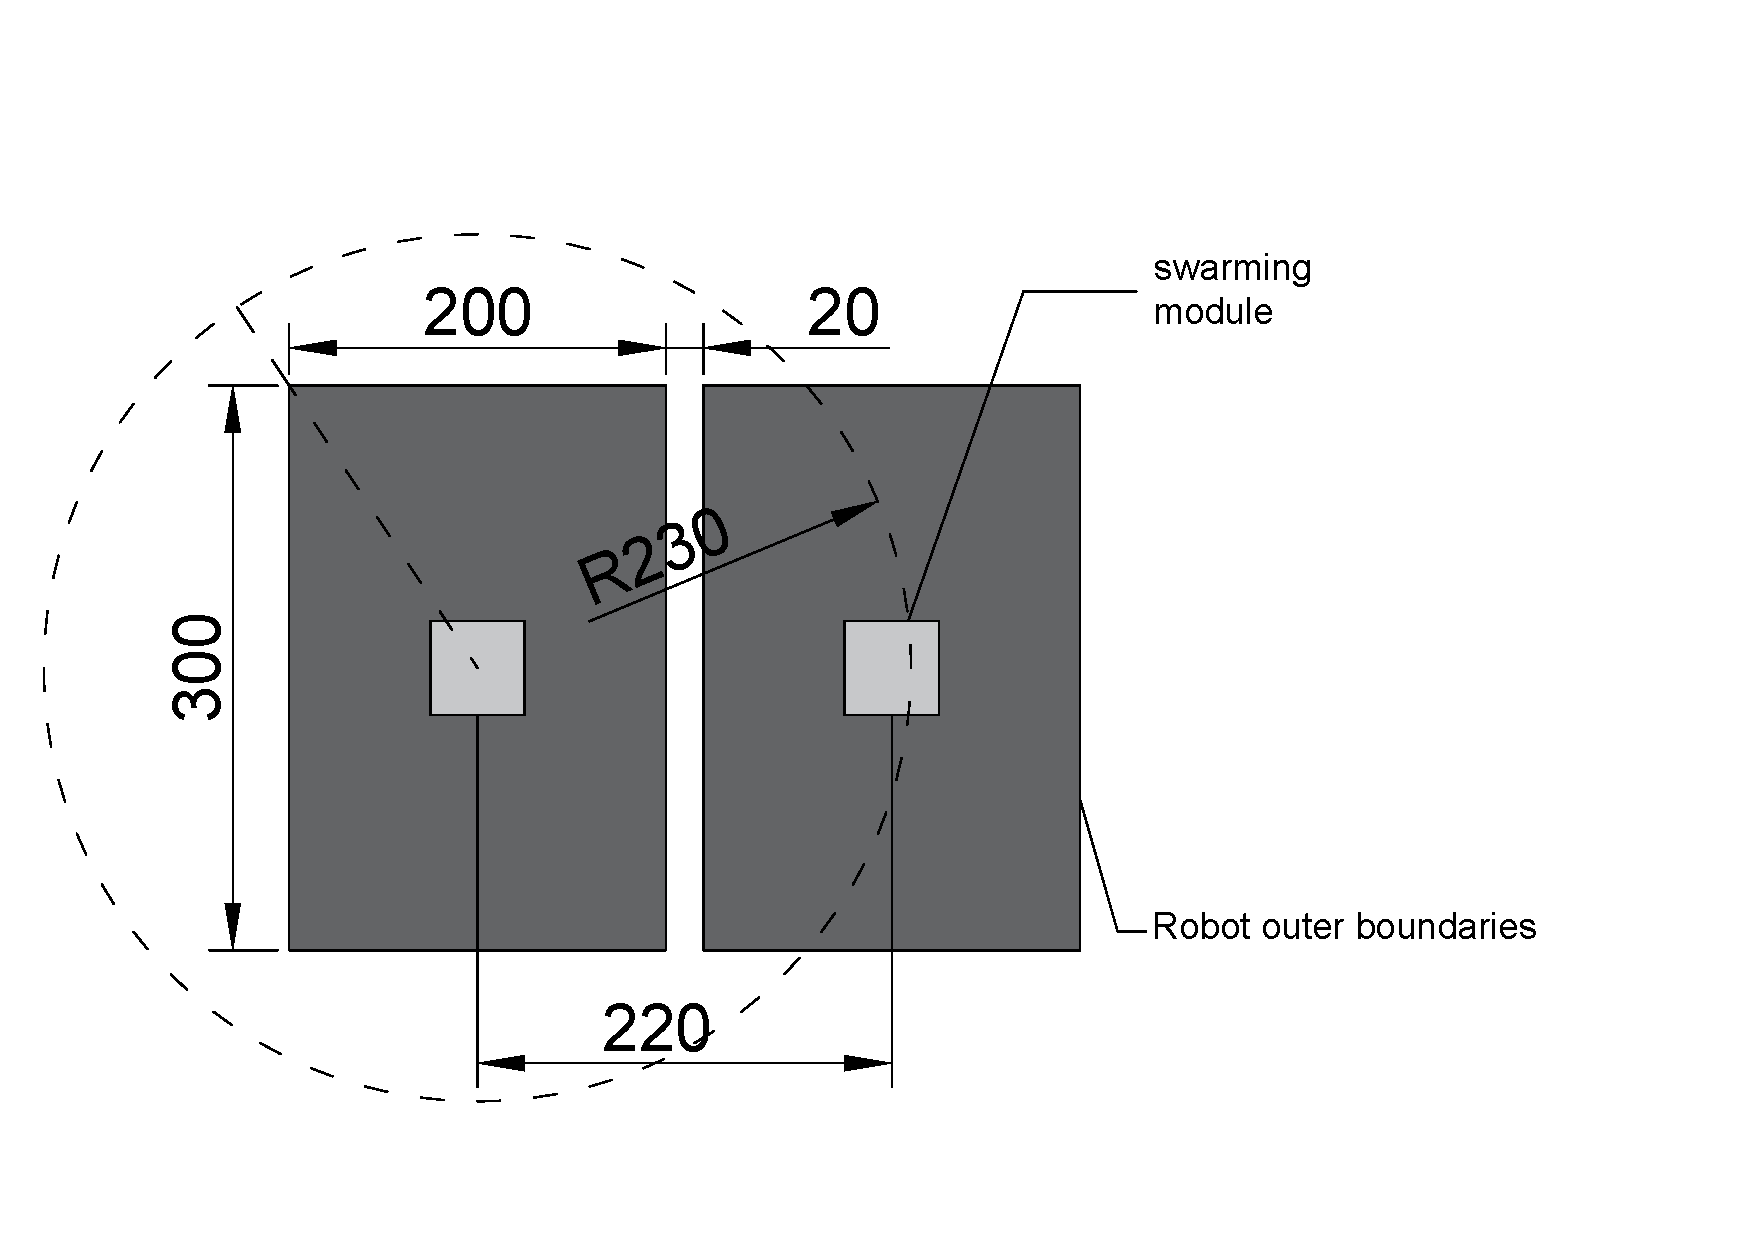
\includegraphics[scale=.3]{smrange.pdf}
        \caption{Worst case scenario for two Zebro light robots at close range}
        \label{fig:smrange}
\end{figure}


Long range localization will only be used to keep members of certain groups in the swarm together. When the units are working together on a task, they will be using the close range localization. A situation might occur where a members of a group of members of the swarm will have to complete a task outside of the range of the close range localization. When they are done and they want to return to the swarm the long range localization will be used. As discussed earlier the long range localization will start at three meters. But it has to get the unit in close range. Therefore the minimal measuring distance will be chosen at two meters. The distance measurement will need to be precise enough to detect when it reaches the overlap between 2 and 3 meters. This maximum deviation for this to be true is 1 meter. Long range localization will actually be a long range distance measurement. The relative angle between modules will not be needed. When an unit needs to return to the rest of the swarm a algorithm can be developed that finds it way back by looking at the changing distance. When the robot is trying to determine the right direction, the update frequency is important. At far range we would assume that a robot has to move one meter to determine if its getting closer or not. With the robot moving at 1 m/s the minimal update frequency is 1 Hz. \\\\
Summed up the specifications of localization are:


% Please add the following required packages to your document preamble:
% \usepackage{graphicx}
\begin{table}[h]
\centering
\resizebox{\textwidth}{!}{%
\begin{tabular}{|l|l|l|}
\hline
                     & \textbf{Close range (0 - 3 m)} & \textbf{Long range (3 - 25 m)} \\ \hline
Dead zone distance    & 0,015 meters                   & 2 meters                      \\ \hline
Deviation (distance) & +/- 9\%                         & +/- 1 meter                   \\ \hline
Angle Resolution     & 45\%                            & -                             \\ \hline
Update frequency     & 40 Hz                           & 1 Hz                           \\ \hline
\end{tabular}%
}
\caption{localization specification}
\label{smrange}
\end{table}



\subsection{Number of units of the Swarm}
As discussed before in the problem definition, its hard to put an exact number on what number of units it required to form a swarm. We mentioned "a high number of units" and that a minimum number of units is hard to justify. We will look at what the preferable amount of units would be to demonstrate the swarming module. Also we will look at a minimum amount and a maximum. Important to remember is that the swarm must always be scalable, so no static number of units will be defined.\\\\Robots in a swarm have limited capabilities on their own, thus they need to work together to perform a complicated task. When one unit breaks down the others should still be able to complete the task. With this is mind the absolute minimum units required for a swarm is chosen to be 3. When one breaks down the other two can still complete the task faster/better than one could do on its own. It would be preferable to make the total swarm endlessly scalable. When developing the swarming module no maximum number should be defined to the swarm. Hardware limitations will later determine a maximum. However a maximum of units can be calculated, that one unit has to be able to detect at close range. The detection surface can be viewed as a circle around of unit with a radius of 3 meters. The radius for the  circle is also calculated for the area where robots will avoid each other. This is done by taking the furthest point seen from the center of the robot and then adding 0,05 m (the range where robots will avoid each other), this circle is shown in figure \ref{fig:smrange}. The maximum amount of robots in this range can then be calculated using a simple tool, the result is shown in figure \ref{fig:ccircle}. The end result is a maximum of 130 robots.

\begin{figure}[H]
        \centering
        \graphicspath{ {./images/} }
        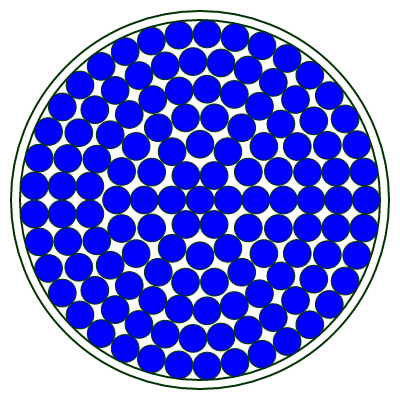
\includegraphics[scale=.6]{ccircle.png}
        \caption{Maximum amount of robots within the close range radius, the maximum amount results in 130.}
        \label{fig:ccircle}
\end{figure}



 For the sake of demonstration we would like to recreate the "feel" of a swarm. This means a higher number of units is required. We chose this number to be between 6 and 12 units depending on the time and budget. 

\begin{table}[h]
\centering
\resizebox{\textwidth}{!}{%
\begin{tabular}{|l|l|l|l|l|}
\hline
 & \textbf{minimum} & \textbf{maximum} & \textbf{maximum (close range)} & \textbf{Preferred (demonstration)} \\ \hline
Number of Units & \multicolumn{1}{c|}{3} & \multicolumn{1}{c|}{$\infty$} & \multicolumn{1}{c|}{130} & \multicolumn{1}{c|}{6 to 12} \\ \hline
\end{tabular}%
}
\caption{Specifications number of units}
\label{specunits}
\end{table}
\newpage

\section{Protocol}
\subsection{Hardware}

For the internal communication between the different systems there are multiple protocols to chose from to transmit data. every subsystem with a microcontroller should be able to communicate with the rest of the system. Because every system should be able to share their information it is necessary to have a multimaster system which allows every system to share their information without being dependent on a single master. To see which protocols are viable multiple protocols will be compared.

Building a modular robot consisting of subsystems, there must be a method to let these "\textit{subsystems}" communicate with each other to exchange relevant information. 

Every subsystem features a micro-controller which must be capable of transmitting and receiving data.  

\subsubsection{TWI}
The name TWI stands for "Two wire interface" which strongly resembles Phillips' protocol $I^(2)C$. Like the name suggests the bus is build up using two wires, one is used for the clock signal and the other is used for the data signal. Each of these wires is connected to the power line through a pull-up resistor so every subsystem connected to the line can pull the line down which other systems can see. TWI can be used as a multimaster system which means every subsystem can send it's data without being dependent on a single master.



\begin{figure}[H]
        \centering
        \graphicspath{ {./images/} }
        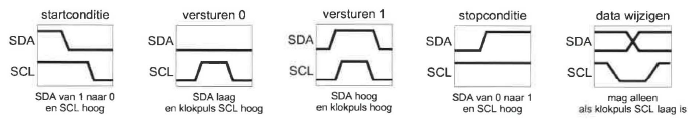
\includegraphics[scale=.6]{datacondities}
        \caption{Data conditions}
        \label{fig:Data conditions}
\end{figure}
In the above figure multiple data and clock combinations are shown, these combinations define the message start, sending a zero, a one and a stop bit. The system that wants to send information starts a message by changing the data signal from one to zero on a high clock signal. All systems that are listening now know one of the systems is going to send a message. Data can be send by changing the data line from zero to one or the other way around during a low clock signal, the other systems will read this bit when the clock signal becomes high again. Once the system is done sending its message it will let the other systems know by sending a stop bit.

\begin{figure}[H]
        \centering
        \graphicspath{ {./images/} }
        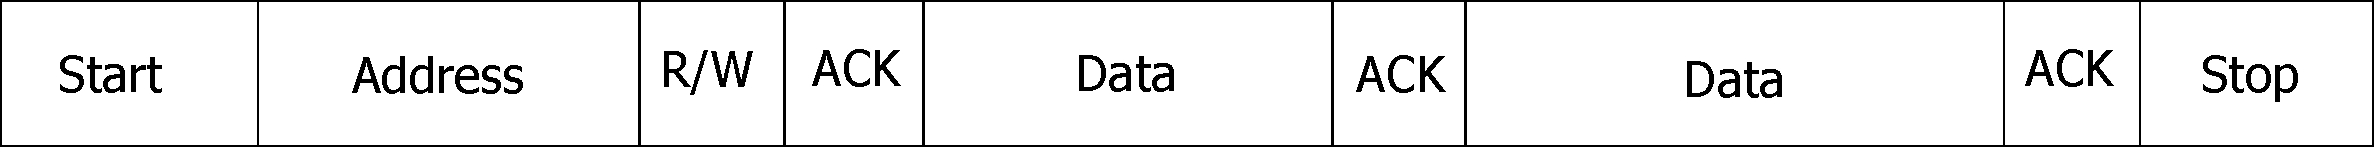
\includegraphics[scale=.3]{TWImessage.pdf}
        \caption{Structure of a TWI message}
        \label{fig:TWIstructure}
\end{figure}
In the above picture the structure of a message is shown. As explained before the message starts with a start bit after which a small header follows. The header contains information about who is going to be addressed by the message and if you want to read or write. After this the addressed system will respond with an acknowledge to make sure the information has come across. When the acknowledge is received the system will start sending data, followed by and acknowledge from the receiver after every received byte of data. when the system is done sending all of its data and received the last acknowledge it will send the stop bit which means all communication has ended.
\\
\\
TWI has a few benefits, because it is a simple serial protocol it only uses two wires. this saves a lot of space in the hardware design. Also, it has the possibility to be used as a multimaster system.
The speed of the communication depend on the frequency of the controller that will be used.


\subsubsection{SPI}
SPI or Serial Peripheral Interface is, like it names suggests, a serial interface. This interface can be connected in two ways, each having its own advantage. How this works will be explained using the following figure.
\begin{figure}[H]
        \centering
        \graphicspath{ {./images/} }
        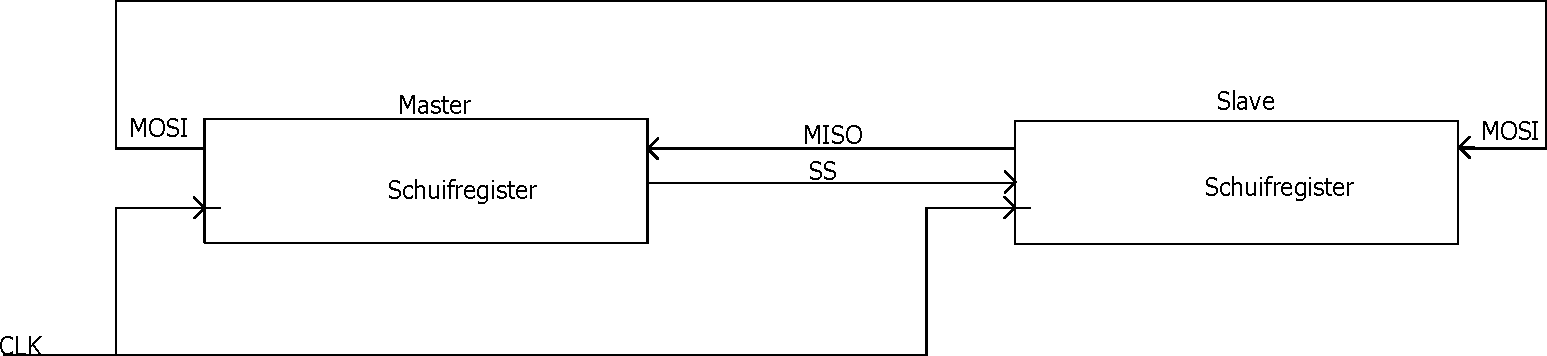
\includegraphics[scale=.4]{SPI}
        \caption{SPI connections}
        \label{fig:SPIconnections}
\end{figure}
SPI works by selecting its slaves using its slave select. Slave select is a single bit used to define which slave the master will be talking to. When the master has selected its slave it will be able to shift its data from its shift register into the shift register of the slave using the MOSI output. MOSI mean master out slave in, so if the master asks data from the slave it will be send using the MISO, master in slave out. Knowing this there are two ways to connect the slaves, putting them in series or parallel to each other. 
\begin{figure}[H]
        \centering
        \graphicspath{ {./images/} }
        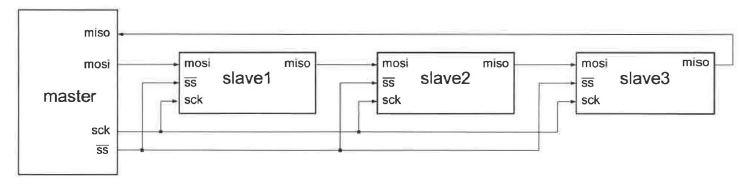
\includegraphics[scale=.4]{SPIserie}
        \caption{SPI connected in series}
        \label{fig:SPIseries}
\end{figure}
When put in series only one slave select will be used to select all the slaves. Each slave will send its data to the next slave through the MISO line. The disadvantage of this method is when you want to address the last slave in line it has to go through all the slaves, meaning it will costs a lot of extra clock ticks to put it through. Another disadvantage of this method is you can not add extra slaves to an existing series of slaves because the path needs to be closed else the slaves will not be able to send their data to the master.
\begin{figure}[H]
        \centering
        \graphicspath{ {./images/} }
        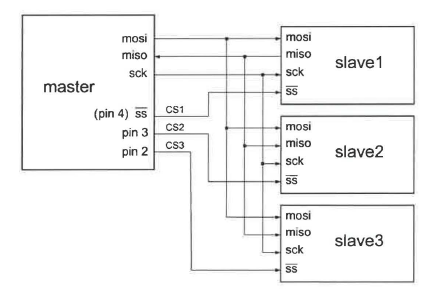
\includegraphics[scale=.4]{SPIparallel}
        \caption{SPI connected parallel}
        \label{fig:SPIparallel}
\end{figure}
The second way to connect the slaves is parallel, this means the master can address all the slaves individually, which will make it faster. The downside of this is you will need a different slave select for every slave. Which means this takes up more outputs from the controller and more space on the circuit boards.
Another downside of SPI is that it can not be used as a multimaster system this downside means it is not viable for the project.
\subsubsection{U(S)ART}
The third serial communication typically used on microcontrollers is U(S)ART. This protocol has two varieties, the universal asynchronous reliever/transmitter and the synchronous. The difference between the two is that the synchronous uses an extra line to send a clock signal. In asynchronous mode the devices synchronise with a start bit at the beginning of the message.
Both of the protocols have a TX and a RX line, the transmit and receive line. Like the name says these are the lines to transceiver the data. Each device connected has two registers, one for receiving data and one for sending. These registers are eight to ten bits long, eight or nine data bits and one or no parity bit. The parity bit can be used as a check to see if the data was received correctly by checking if the amount of ones is even or odd. The message is ended with one or two stop bits. So a typical U(S)ART frame looks like the figure below.
\begin{figure}[H]
        \centering
        \graphicspath{ {./images/} }
        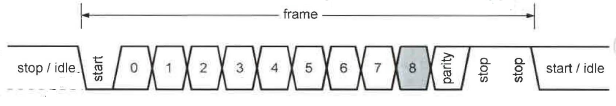
\includegraphics[scale=.4]{UARTframe}
        \caption{Typical U(S)ART frame}
        \label{fig:UARTframe}
\end{figure}
Depending on the software protocol used it is possible to have a multimaster system using one U(S)ART connection on every device. Every message should get a header in which the addressed device is selected.

\subsubsection{Conclusion}
Looking at the specifications of each protocol and comparing those, there can be concluded that TWI is most suitable. This is because of the fact it only uses two lines to communicate and is easily implemented in a multimaster system.


\subsection{Software}


\newpage
\section{Localization}
Building a swarm of robots, location awareness may be required to ensure an more efficient operation. Implementing location awareness into a swarm of robots could result in better cooperation. For example: exploration based tasks can be executed on a much lower time scale. With location awareness the swarm can spread out evenly making sure that every part of the perimeter will be explored thoroughly. 

With location awareness it is also possible to divide the swarm into multiple groups. Because the location of every individual is available these individual groups can be formed very quickly by selecting the nearest unit. This also enables quick assists when an individual robot gets stuck or needs to execute a task that requires more than one unit.

For mapping the various positions of all robots in a swarm a localization technique needs to be implemented. The robots can use information as relative position and relative orientation of their neighbours and fuse the information collected by other robots to interpret the relative location. With relative position the units can define the distance relative to each other. When all robots in the swarm are aware of the distance opposite to each other, a map of the current formation can be created. However this can result in multiple solutions because there are no orientations involved. 

\subsection{Angle determination}
Determining the relative orientation with respect to each other can be done in various ways. some methods involve larger limitations than others. In general angular measurements are done using goniometric equations.

\subsubsection{Goniometric angle determination}
The goniometric system shows how the different angles of a triangle within a circle can be calculated. Determining angles of a triangle within a circle using goniometric formulas, a mirroring phenomenon can occur this happens because of the following relation between the angles see figure \ref{circle}. This mirroring will be explained in more detail below.

\begin{figure}[H]
\centering
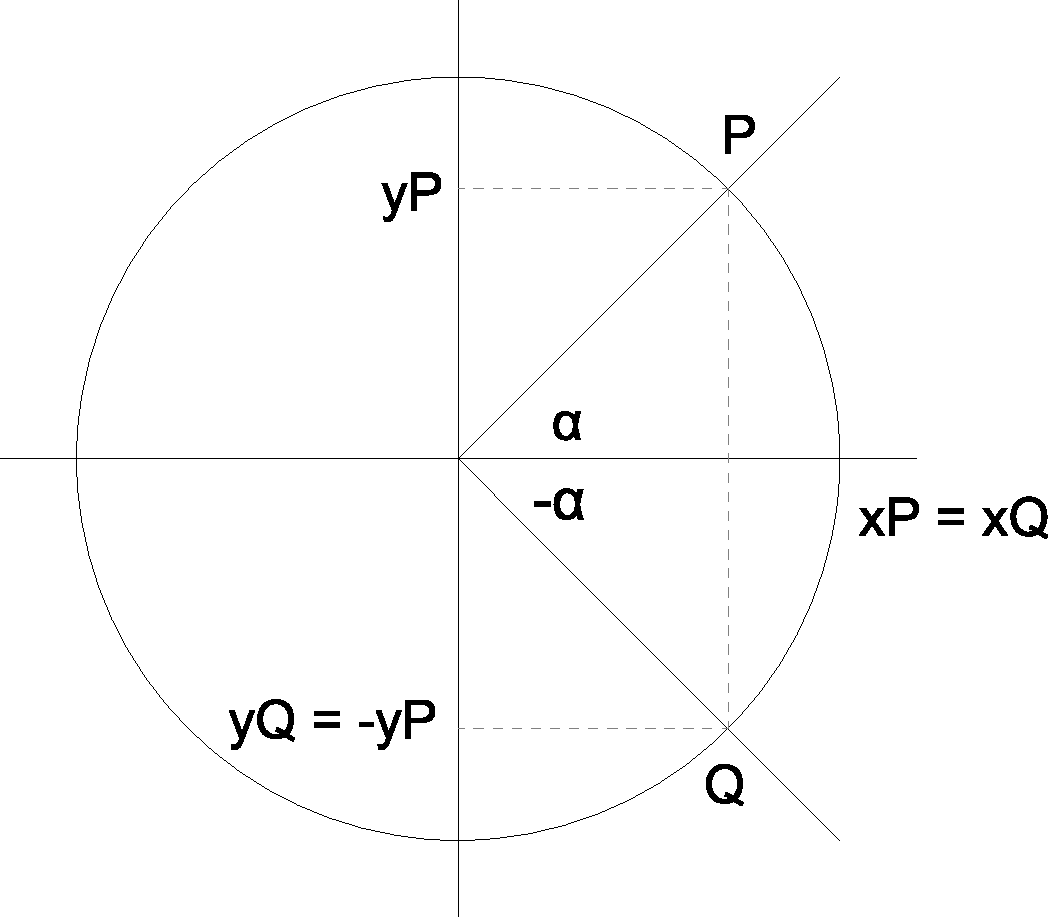
\includegraphics[width=0.7\textwidth]{Cirkel.pdf}
\caption{Unit circle where points P and Q are mirrored on the X-axes}
\label{circle}
\end{figure}

\begin{equation}
Because\ Xp = Xq,\ cos(-\alpha) = cos(\alpha)\ applies
\end{equation}

\begin{equation}
Because\ Yq = -Yp,\ sin(-\alpha) = -sin(\alpha)\ applies
\end{equation}

This mirroring phenomenon is something that needs to be resolved. Mirroring of the angle means that the robot(s) which is being detected could be in two different direction relative to the interpreter. Figure \ref{detectie} shows how the different robots determine the relative distance to each other. 

\begin{figure}[H]
\centering
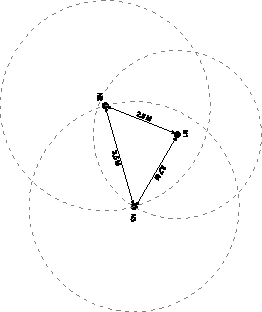
\includegraphics[angle=90,width=0.7\textwidth]{Detectie.pdf}
\caption{Relative location interpretation}
\label{detectie}
\end{figure}

In figure \ref{detectie} a scenario is given where the relative distance between the different nodes (N1, N2 \& N3) is known but their position within the circle is unknown. According to the goniometric equations the direction (angle) within a circle could be mirrored as shown in equation 1 and 2. This could lead to two different interpretations one being the reality as shown in figure \ref{mirror} and one being mirrored as shown in figure \ref{mirror1} (where N1 is the interpreter). 

\begin{figure}[H]
\centering
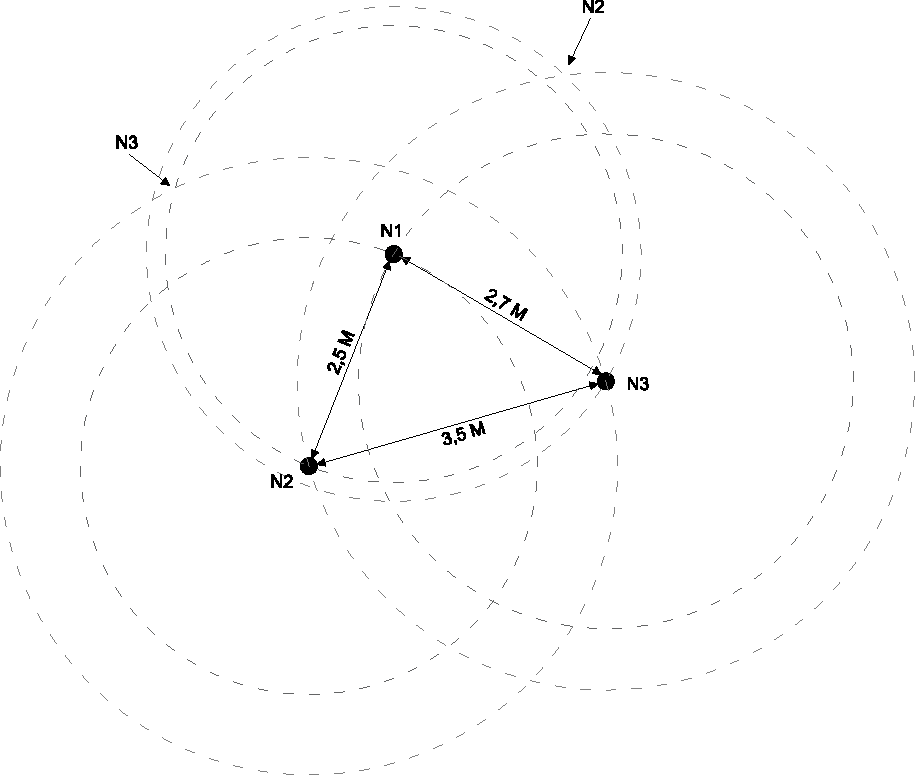
\includegraphics[width=0.7\textwidth]{Mirror1.pdf}
\caption{N1 Location interpretation}
\label{mirror}
\end{figure}

In a more practical scenario instead of a mathematical scenario this mirroring phenomenon occurs because every node draws a circle towards the detected node. Doing so this leads to two different intersectionpoints, one being the "real" position and one being the mirrored opposite. In figure \ref{mirror} the real position is shown, also the intersections of the different circles are displayed. Each intersect is a potential location of a node, as seen in figure \ref{mirror} per node there are two possibilities. In figure \ref{mirror1} the mirrored interpretation of N1 is illustrated.
 
\begin{figure}[H]
\centering
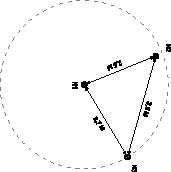
\includegraphics[angle=90,width=0.7\textwidth]{Mirror.pdf}
\caption{N1 Mirrored interpretation}
\label{mirror1}
\end{figure}

For the robots to know in what direction the measured distance is applicable to, they can analyze the change in distance after a robot has moved a specific direction. In order to leverage the previous trilateration procedure requires coordinating the motion of the robots in a manner that gives every robot a chance to move and ensures that when a robot is moving its neighbours remain stationary. \cite{Angle}

This method is very impractical because several robots need to abort their current task to move around. This method takes a lot of time to complete and therefore angular updates cannot be done very often. For previous research in this specific field, determining oriantation with movement see \cite{delft}.

This can also be achieved by the use of stationary beacons. When a minimum of three beacons is placed on the field the location of the robots within this field can be measured, this is called triangulation. Triangulation is the process of determining the location of a point by measuring angles to it from known points. This is illustrated in figure \ref{driehoek}.

\begin{figure}[H]
\centering
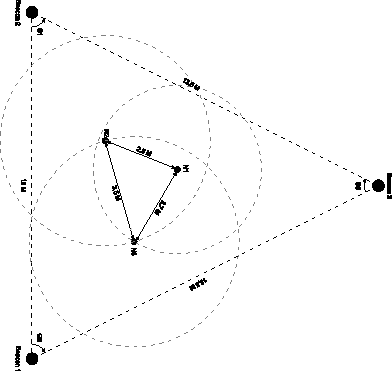
\includegraphics[angle=90,width=0.7\textwidth]{driehoek.pdf}
\caption{Triangulation using three stationary beacons}
\label{driehoek}
\end{figure}

Using three stationary beacons the exact position of every node within this field can be calculated. This can be done by using the cosine rule shown in the equations below. 
\begin{equation}
A^2 = B^2 + C^2 - 2\cdot B\cdot C\cdot cos(\alpha)
\end{equation}

\begin{equation}
B^2 = C^2 + A^2 - 2\cdot C\cdot A\cdot cos(\beta)
\end{equation}

\begin{equation}
C^2 = A^2 + B^2 - 2\cdot A\cdot B\cdot cos(\gamma)
\end{equation}

With the cosine rule exact location of the different nodes can be determined. Using three stationary beacons mirroring cannot occur any more. Because if one beacon measures a distance to a node that is greater than the mutual-distance to another beacon the node is no longer located within the triangulation field.

\begin{figure}[H]
\centering
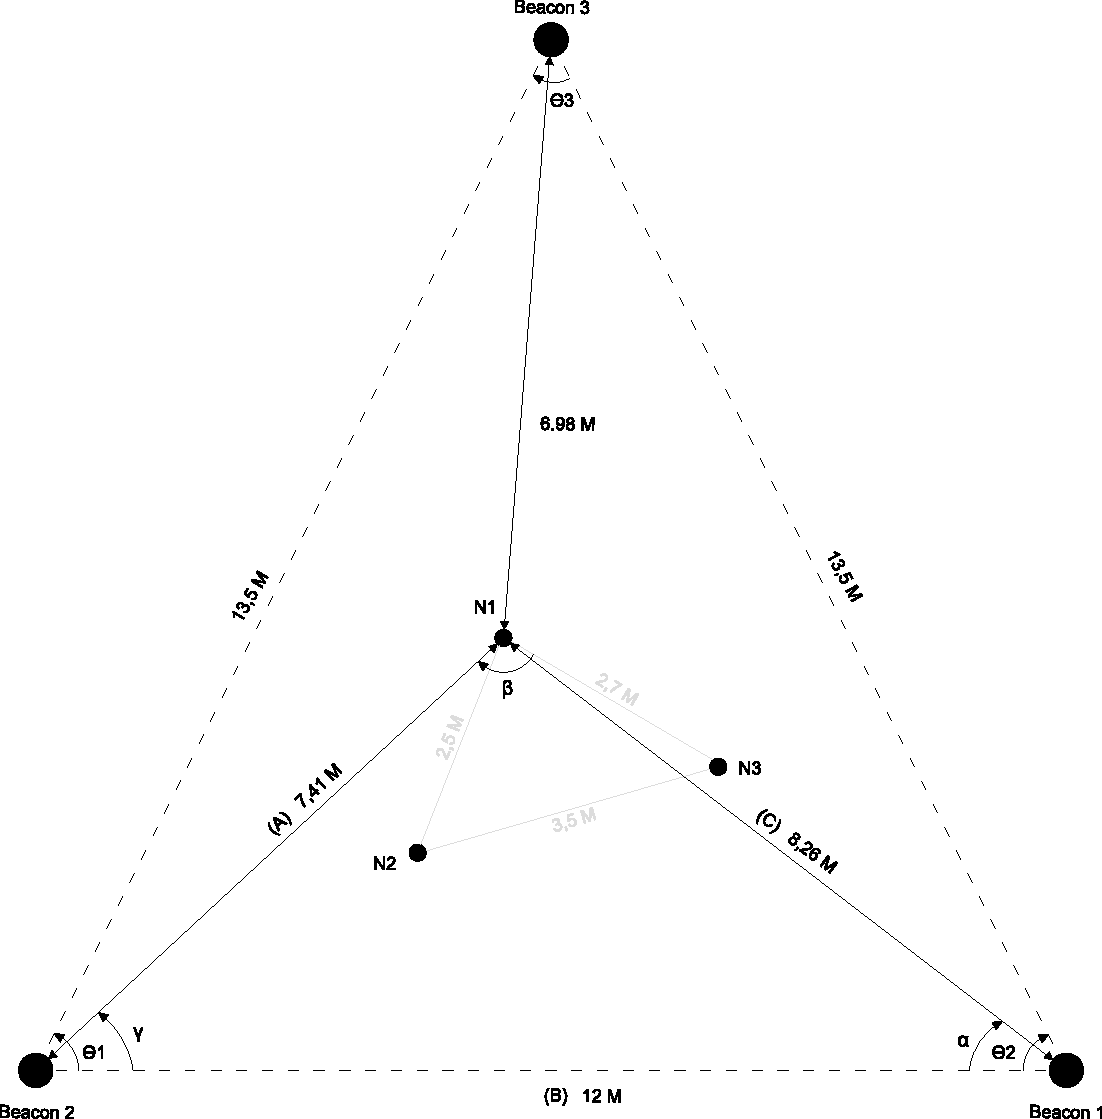
\includegraphics[width=0.6\textwidth]{triangulatie.pdf}
\caption{Determining the angle with three stationary beacons}
\label{triangulatie}
\end{figure}

In figure \ref{triangulatie} the distances from the beacons to node 1 (N1) are being determined. With these distances the different angles can be calculated this is done in the equations below.

\begin{equation}
A^2 = B^2 + C^2 - 2\cdot B\cdot C\cdot cos(\alpha)
\end{equation}

\begin{equation}
\label{eq:hoek}
cos(\alpha) = \frac{(B^2 + C^2 - A^2)}{(2\cdot B\cdot C)}
\end{equation}

\begin{equation}
\label{eq:hoek}
\frac{(12^2 + 8,26^2 - 7,41^2)}{(2\cdot12\cdot8,26)} = 0,7935
\end{equation}

\begin{equation}
cos^{-1}(0,7935) = 37,48\degree
\end{equation}

The equations above results in a vector (C) pointing towards the node. doing this for every line (A,B \& C) results in three vectors, all three pointing towards the node from different origins, this leads to the exact location of the node. 

Implementing localization using three stationary beacons involves several limitations to the swarm. These limitations are that the swarm cannot operate far away from the triangulation field and therefore is limited to a specific perimeter, because if the units move to far away from the beacons they become out of range. Also spreading three stationary beacons autonomously is a difficult task to accomplish.  

A more efficient solution is to retrieve the relative orientation opposite to each other. In combination with the relative distance every robot knows the exact relative position of all the other robots in range of the network.

\begin{figure}[H]
\centering
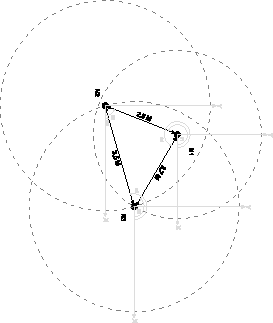
\includegraphics[angle=90, width=0.6\textwidth]{orientation.pdf}
\caption{relative localization system using relative distance and orientation}
\label{orientation}
\end{figure}

As seen in figure \ref{orientation} each node has a common reference direction (X,Y), the direction relative to this reference is called the relative orientation of the robot and can be visualized as shown in figure \ref{orientation}. This relative orientation can be achieved using a compass of some sort. With the known distances, the mapping of the swarm can be completed.
\newpage

\subsubsection{Trigonometry}
Another method of angle determination is using trigonometry. With trigonometry there is no mirroring due to the fact that all the circles only intersect at one point see figure \ref{trigonometry}. The base functionality of trigonometry is based upon triangulation, except of implementing three stationary beacons on the ground the beacons are placed in one mobile module placed upon a node (robot) for example.

\begin{figure}[H]
\centering
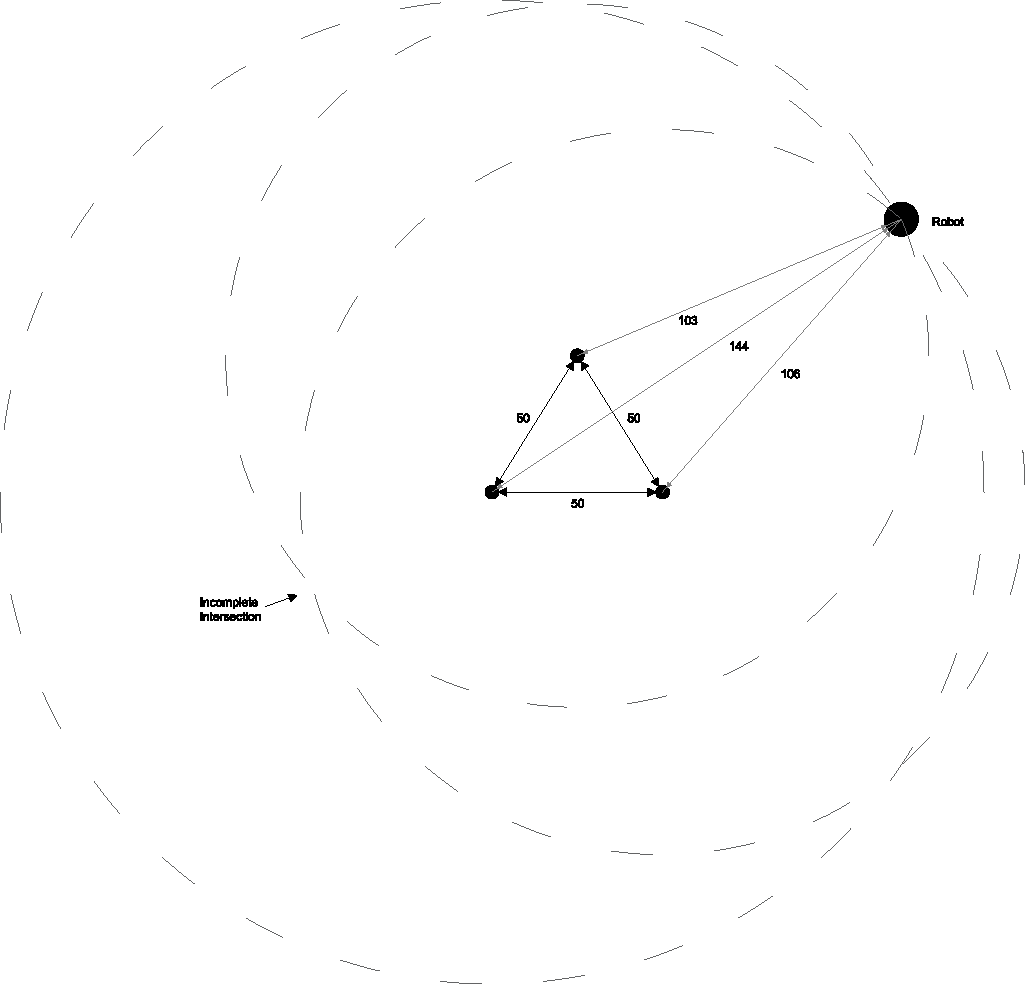
\includegraphics[width=1\textwidth]{trigonometry.pdf}
\caption{Angle determination using trigonometry}
\label{trigonometry}
\end{figure}
\newpage

\subsection{Relative Distance}
Relative distance can be measured using various methods. The most common methods are \textit{"Received Signal Strength Indication"} and \textit{"Time Of Flight"} abbreviated as RSSI and TOF. 

\subsubsection{Received Signal Strength}
A method to determine distance can be implemented using Received Signal Strength abbreviated as "RSSI". Typically RSSI of WIFI is a measure of dBm, which is ten times the logarithm of the ratio of the power (P) at the receiving end and the reference power (Pref). Power at the receiving end is inversely proportional to the square of distance.\cite{RSSI} Hence RSSI could potentially be used as an indicator of the distance at which the sending unit (robot) is located from the receiving unit.\cite{RSSI}

In theory it seems as a suitable implementation for the purpose, determining relative distance between different units. However various test results have shown that RSSI is only reliable under certain circumstances. Test results have shown that if the orientation of the sending or receiving unit changes it becomes very unreliable. The graphs below show the reliability of RSSI when the direction is being altered.\cite{RSSI}

\begin{figure}[H]
\centering
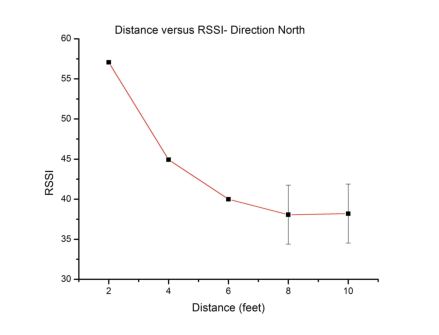
\includegraphics[width=0.9\textwidth]{North.pdf}
\caption{Distance versus RSSI plot showing inverse non linear
relationship.\cite{RSSI}}
\label{North}
\end{figure}

\begin{figure}[H]
\centering
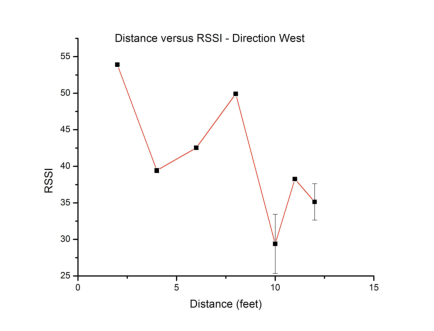
\includegraphics[width=0.9\textwidth]{West.pdf}
\caption{Distance versus RSSI plot showing lack of
reliability when tested in a different direction.\cite{RSSI}} 
\label{West}
\end{figure}

\begin{figure}[H]
\centering
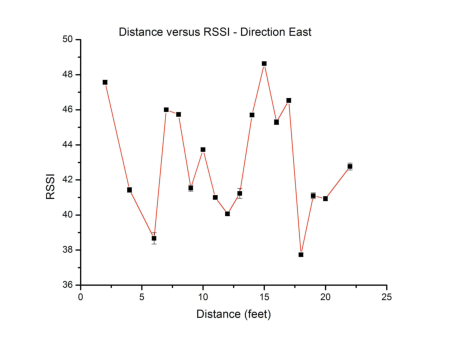
\includegraphics[width=0.9\textwidth]{East.pdf}
\caption{Distance versus RSSI plot showing lack of
reliability when tested in a different direction.\cite{RSSI}} 
\label{East}
\end{figure}
\newpage


Even though RSSI was very promising in many studies, through multi directional experiments it became clear that even under ideal conditions with weather and interference controlled, the RSSI data could not be relied upon. At times the data was correct showing the expected inverse square relation with distance and at other times it didn't.\cite{RSSI}


\subsubsection{Time Of Flight}
Another common method to determine relative distance is Time Of Flight abbreviated as "TOF". Time Of Flight describes a method that measures the time that an particular wave takes to travel a distance trough a medium. The wave can be acoustic, electromagnetic and light.

For relative distance measurements Time Of Flight is often combined with Time Difference Over Arrival abbreviated as "TDOA". Combining these methods enables relative distance measurements to specific units/nodes. TDOA measures the time difference between the transmission and arrival of a wave. With the velocity of propagation times the travelled time the relative distance between two or more nodes can be determined. However TOF also features certain limitations being clock synchronization, noise, sampling and multipath channel effects.\cite{TOF} Where the most important limitations for our purpose are clock synchronization and sampling, which will be addressed below.
\\\\
\textit{Clock Synchronization}
TOF ranging systems need to estimate the time of transmission and arrival and comparing this with a common time reference.\cite{TOF} If the different time references are not perfectly synchronized a time offset error occurs. With the faster the propagation speed, the greater the error in distance. 
\\\\
\textit{Sampling}
Using Light or electromagnetic waves to determine the relative distance can add several limitation. Due to the high velocity propagation (being nearly equal to equal of the velocity propagation of light) sampling this signal requires very high clock rates to do so. It would take a 15GHz clock to achieve one centimetre resolution.\cite{Arduino}

in the 1960's, Tektronix invented a sampling method with a oscilloscope that could measure signals in the GHz range without using high speed clocks. This method is called Sequential Equivalent Time Sampling abbreviated as "SETS". The SETS acquires one sample per trigger see figure \ref{SETS}. When a trigger is detected a sample is taken after a very short, but well defined delay. When the next trigger occurs a small time increment "Delta T" is added to this delay and the digitizer takes another sample. This process is repeated many times with "Delta T" added to each previous acquisition, until the time windows is filled.\cite{SETS} In figure \ref{SETS2} another example of an sinusoidal signal is displayed using the SETS method. 

Using the SETS method enables the use of waveform with an velocity propagation nearly equal to equal to the speed of light. However implementing an advanced SETS circuit is required to reach accuracy of less than 1 meter indoors.\cite{TOF} The benefit of waveforms with a high velocity propagation is faster data transfers and a larger range.\cite{TOF} Even though the SETS method seems as a suitable solution for the problem it is only functional for repeating signal patterns. It is possible to "see" that a signal has been received, but its unable to determine a "time stamp" of the signal.

\begin{figure}[H]
\centering
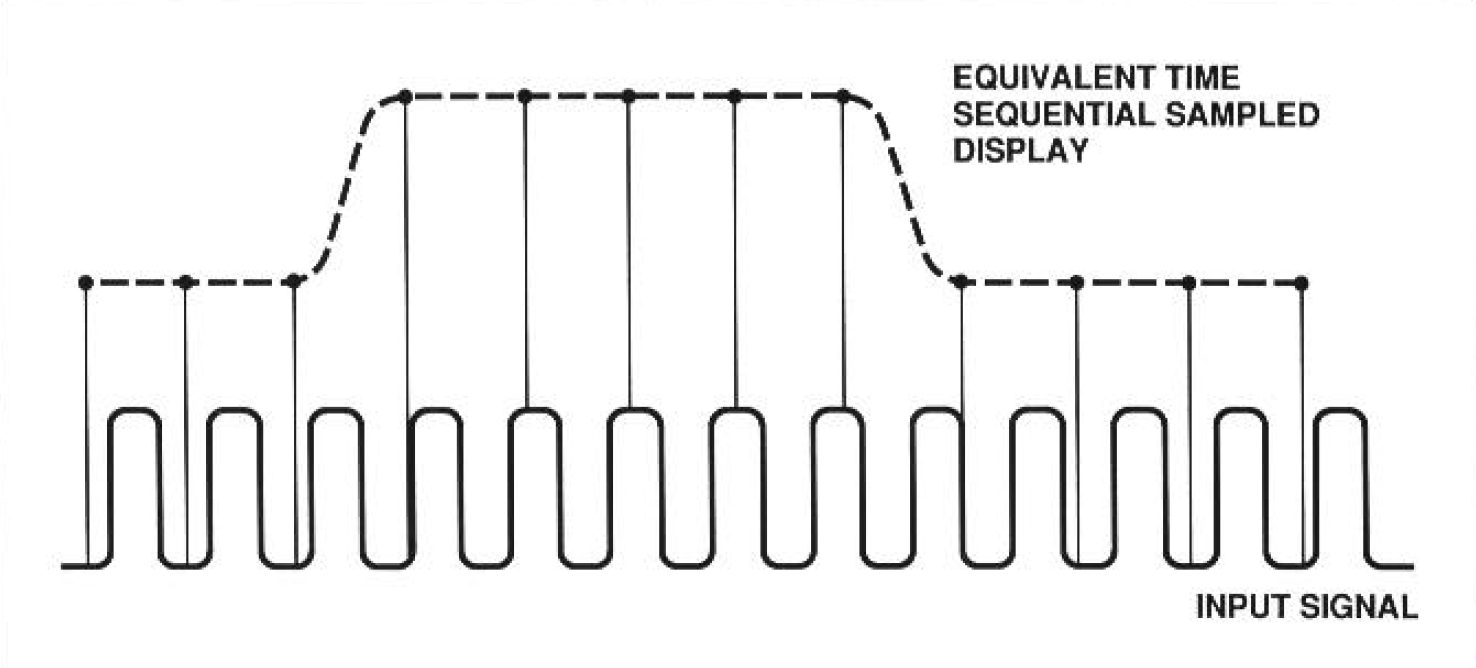
\includegraphics[width=0.9\textwidth]{SETS.png}
\caption{In sequential equivalent time sampling a single sample is taken for each recognized trigger after a delay which is incremented after each cycle.\cite{SETS}} 
\label{SETS}
\end{figure}

\begin{figure}[H]
\centering
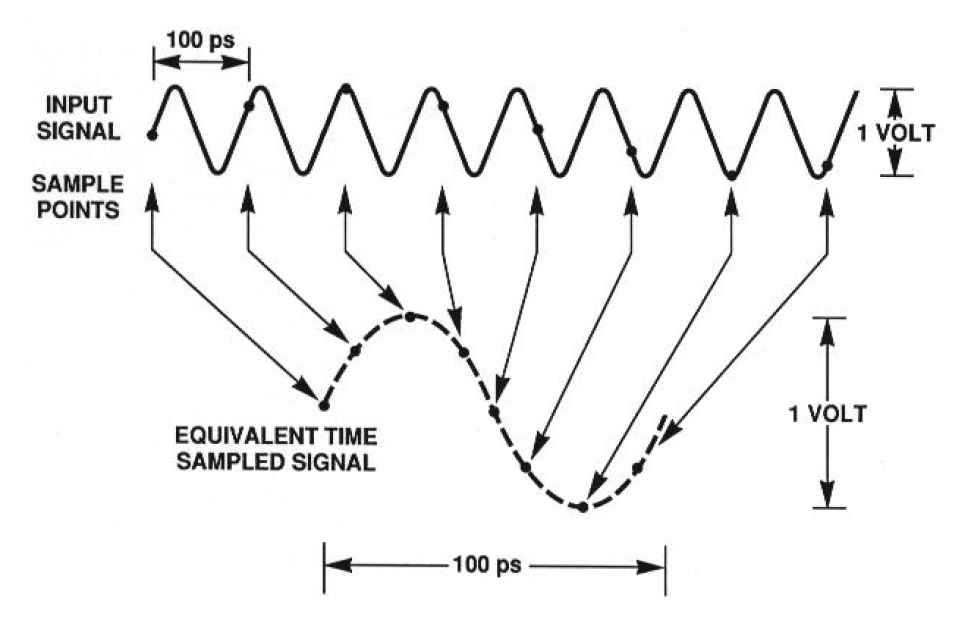
\includegraphics[width=0.9\textwidth]{SETS2.png}
\caption{Example equivalent time sampled signal.\cite{SETS}} 
\label{SETS2}
\end{figure}
\newpage

\subsection{Localization conclusion}
Different studies have shown that Received Signal Strength can theoretically measure distance accurately. However RSSI seems to be very unreliable in many circumstances which leads to not being viable for distance measurements with moving robots. 

Time Of Flight has been very promising, however using electromagnetic signals (For example RF, WI-FI or Bluetooth) the acceptable accuracy starts at from a minimum range of 1-2 meters which leads to unreliable to no useful information at all in the range of 1-2 meters. This minimum range could be narrowed using an Sequential Equivalent Time Sampling Circuit, however such a circuit is complex to develop. However using waveforms with a lower velocity propagation can lead to accurate close range measurements. In this case Time Of Flight suits better for the required use, being more accurate and reliable see figure \ref{RSSIvsTOF}.\cite{TOF}

\begin{figure}[H]
\centering
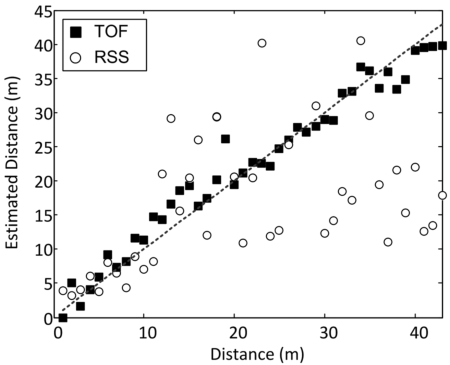
\includegraphics[width=0.9\textwidth]{RSSIvsTOF.pdf}
\caption{Accuracy RSSI vs TOF.\cite{TOF}} 
\label{RSSIvsTOF}
\end{figure}

Determining relative distance does not lead to localization. To do so an angle is required. Angle determination can be done in various ways, most of them implementing the goniometric system. The goniometric system explains different approaches for determining the relative angle. The most common method is determining relative location with the use of three stationary beacons, however this limits several possibilities of the entire swarm, being limited to the triangulation perimeter and autonomous spreading the beacons is a difficult and time consuming task.
Another method is determining relative angle using movement. While measuring the relative angle a phenomenon called mirroring will occur where the angle of the detected node can be in two different directions, one being the reality and one being mirrored. This phenomenon needs to be resolved, and can be done by moving the nodes in different directions after the first measurement has been done. After the first measurement cycle has been completed, the nodes have to move in a specific location then a second measurement cycle measures the movement of the node relative to the first measured location. Doing so this will eliminates the mirrored angle and the relative angle remains. However determining relative angle using movement techniques is a time consuming task and therefore angular updates cannot be done very often.
However trigonometry seems very promising, since mirroring phenomenons cannot occur any more angular determination can be done without major obstacles. Also with the use of trigonometry it is also possible to determine the distance towards a node. Combining the two measurements should lead to a relative localization.

\newpage

\section{Acoustic sensing}

Relative distance sensing can be done by simultaneously sending an RF signal and a sound wave and subtracting the time of arrival.
This method of sensing is based on the fact that RF signals travel with the speed of light and thence travels much faster than sound through the atmosphere: Light travels at 299.792.458 m/s, whereas the speed of sound is only about 332 m/s, depending on air temperature:
\begin{equation}
\label{eq:speedsoundinair}
V_{sound in air}(m/s)\approx 331.4+0.6T_{c}
\end{equation}
Since the speed of the RF signal is so much faster than the speed of sound, the time of arrival of the RF signal in this situation is negligible. Which leads to the following formula:
\begin{equation}
Relative distance(m) \approx Toa_{sound}(s)\cdot  331.4+0.6T_{c}
\end{equation}
Distance measurement by acoustic signals using time of flight could be a good option for short range localization between 0 and 3 meters. A couple of test where done to test if measuring time of flight of sound waves is suitable for a swarming application. the following points need to be researched:
\begin{itemize}
\item To complement the shortcomings of the far range localization system the signal needs to be able to travel atleast 3 meters.
\item Because the robots need to create awareness to all other robots around, it is important that the waves travel omnidirectional. 
\item To make the localization as accurately as possible there needs to be a minimum of interference. 
\end{itemize}

\subsection{Frequency ranges}
The speaker used for these test has a frequency range between the 130 Hz and 20 kHz. To test what the influence of different frequencies is on the distance that the waves can travel figure \ref{setup1} shows the test set-up used.

\begin{figure}[H]
\centering
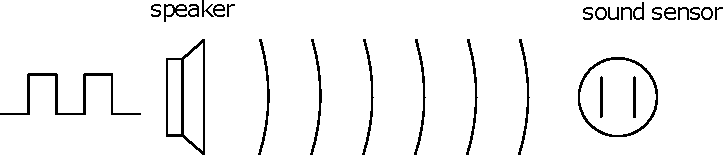
\includegraphics[width=0.9\textwidth]{situation1.pdf}
\caption{Setup used to test the range of different frequencies} 
\label{setup1}
\end{figure}

The speaker is faced directly at the microphone to create an ideal situation. 

The higher frequencies are better visible then the lower frequencies. That could be explained by the fact that the higher frequencies contain a lot more energy in the more bundled wave form. If the waves are used in a specific direction a higher frequency is more preferable.  

\subsection{Wave characteristics}

To test the spread of the sound waves the speaker was placed on the table facing upwards. On a distance of 1 meter we placed a microphone, also facing upwards, which was connected to an oscilloscope as shown in figure \ref{setup2}. The microphone was moved away from the speaker every time the signal was clear. This way the maximum distance for the frequency could be determined. The maximum range needed is 3 meters. For each frequency we tested what the microphone was picking up and how the signal showed up. 

\begin{figure}[H]
\centering
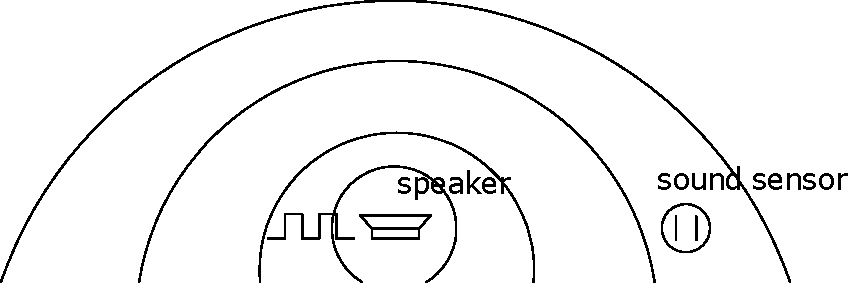
\includegraphics[width=0.9\textwidth]{situation2.pdf}
\caption{Setup used to test the omni-direction range and wave characteristics} 
\label{setup2}
\end{figure}

From 100 Hz to 1 kHz no signal could be detected, even when the microphone was placed very closely. From 2 kHz to 4 kHz the signal became very clear. Although there where some situations where the signal was not as clear as all other situations. These frequencies where loud and clear at a distance of 3 meters. Above the 5 kHz the sounds became a lot more directional. The microphone did not sense any of the waves, unless the speaker was directly aimed at the microphone. 
 
There are ways to manipulate the direction of the sound waves. If there is need to use higher frequencies. By the use of a parabolic reflector a higher frequency sound beam can be converted to a more omnidirectional wave. 

Some experimental tests where done with a parabolic reflector. In this case a square of aluminium placed slightly above the speaker. The results where promising. The signal was a lot smoother and had more amplitude then before. The frequency waves between 3-5 kHz acted a lot more omnidirectional. The higher frequencies 5 kHz and above could not be sensed by the microphone even with the aluminium plate placed above the speaker. For now it seems that the characteristics of the frequencies between the 3 and 4 kHz meet the requirements.

\subsection{Experiment Sensor}

From the previous experiment a suitable frequency range was chosen. In the following experiments we tested what the microphones would pick up if they where only 5 centimetres apart from each other. It is important that the direction of the signal can be determined by analysing where the sound wave entered first. But this is only possible if the smallest change in distance can be detected as well. 
The set up was as followed: We placed a speaker about 1 meter from the microphones. The microphones where placed in three different kind of set ups. In the first set up the microphones where placed side to side. If the sound is transmitted it should not give a different signal on the microphones since the distance from the speaker to the sensor is equal. 
In the second set up, we turned the microphones so that one of the microphones was slightly further away from the sound source. In the third set up the microphones where behind each other with a distance of 5 centimetre. If we want to determine the location it is necessary to determine where the sound will be detected first.  
The results where as to be expected. The output of the microphones are connected to the oscilloscope. 

\begin{figure}[H]
\centering
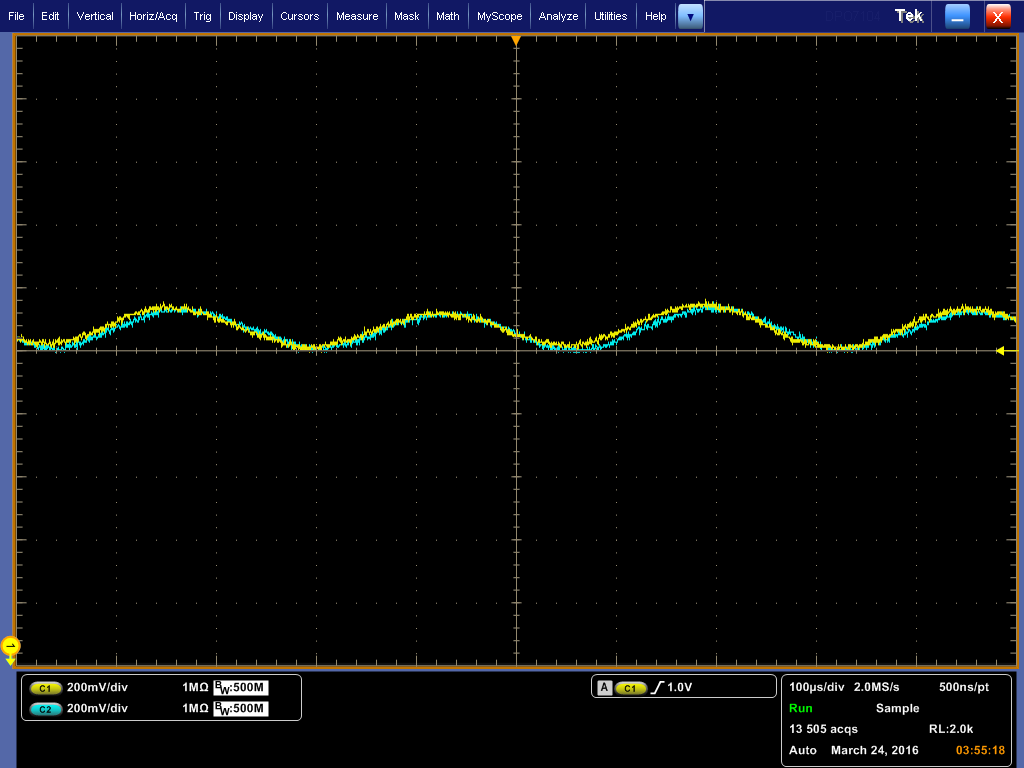
\includegraphics[width=0.9\textwidth]{experiment1.png}
\caption{Result with two microphones at the same distance} 
\label{experiment1}
\end{figure}

There is almost no difference between the two signals , that means that both sensors received the sound on the same time. 

\begin{figure}[H]
\centering
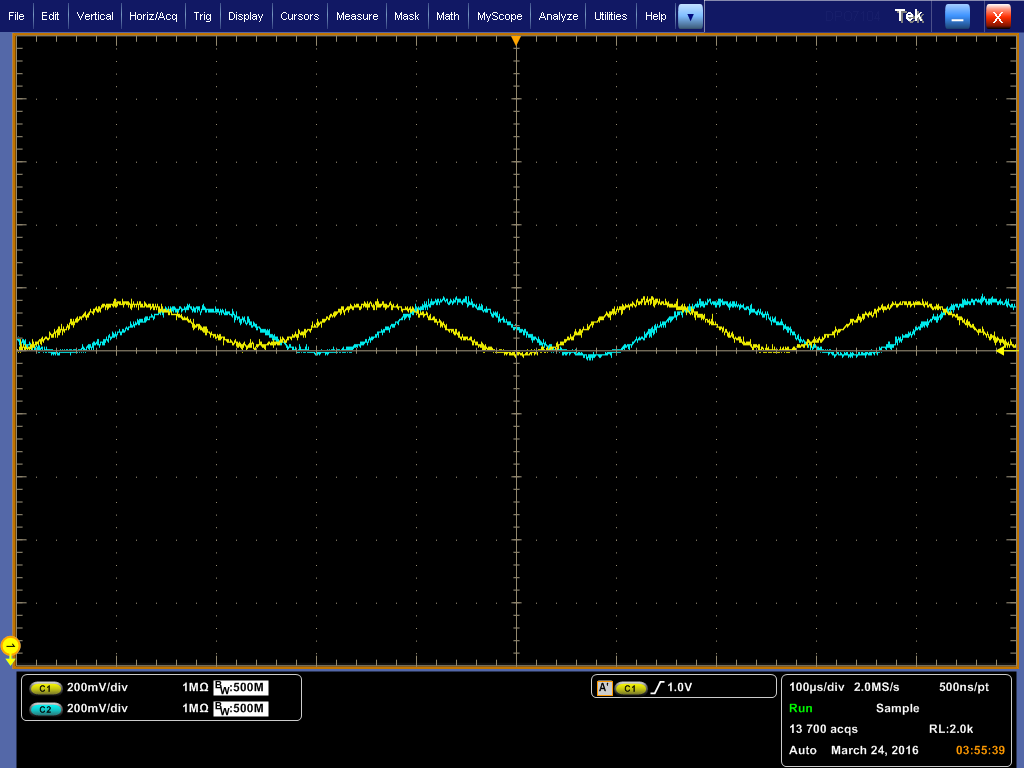
\includegraphics[width=0.9\textwidth]{experiment2.png}
\caption{Result with one microphone slighty further} 
\label{experiment2}
\end{figure}

The microphone was not placed that much further but the result shows very clearly that it there is a phase shift between the signals.
From this experiment can be concluded that short distance localization is possible, since the signals can easily be distinquised. 
\begin{figure}[H]
\centering
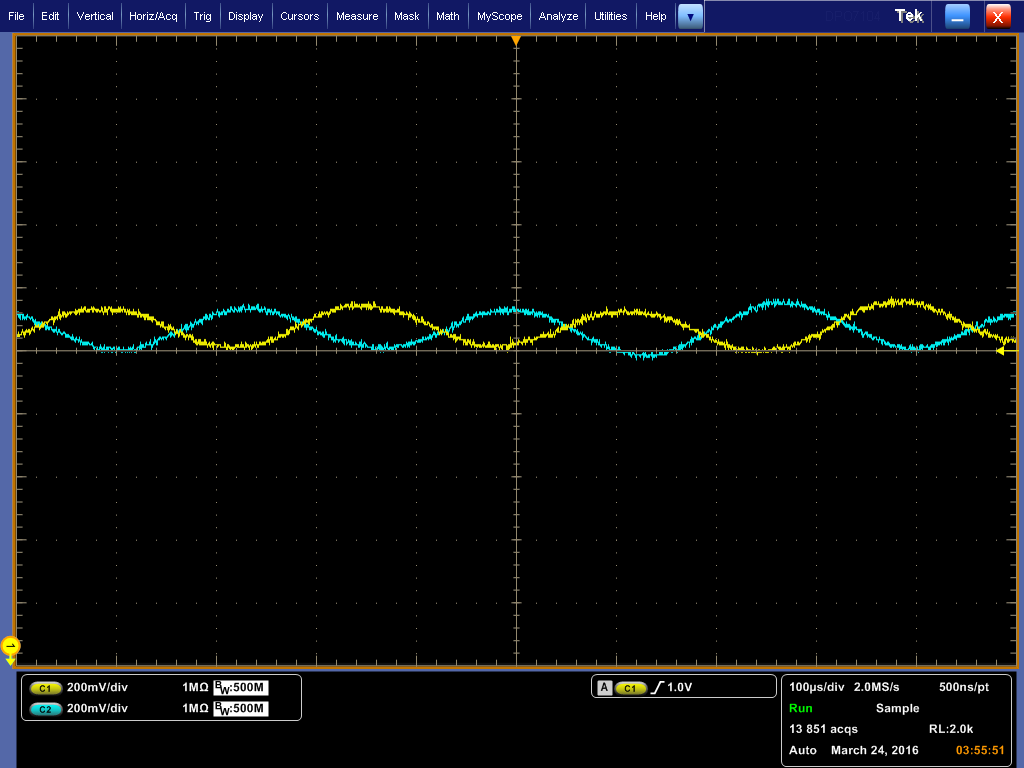
\includegraphics[width=0.9\textwidth]{experiment3.png}
\caption{Result with one a distance of 5 centimetres between the microphones} 
\label{experiment3}
\end{figure}

With the microphone placed even further away the phase shift increases. The results are as expected, and this experiment shows that even small distances can be distinguished with this method.

\subsection{Interference}

Until now only the travel characteristics where tested, but how does the environment have effect on these sound waves. Are the lower or the higher sound waves more more influenced by noise. And if so, can the noise be minimized with filtering. Most of the noise between the frequencies between 100 Hz and 20 kHz will come from human speech. In a demonstration sources like music or noise from outside could be minimized, but speech inside a room is hard to ignore. If a band-pass filter is implemented a lot of frequencies can be filtered out depending on how well the filter is build. Experimenting with this set-up is needed to determine if a filter will suffice.

\subsection{Modulation}

Another way to distinguish the sound waves from the noise, is to modulate the sound waves. If some sort of information is implemented on the sound wave it could be recognized and be distinguished from the noise. Another advantage of this method is, that it is possible to send information. Since the speed of sound is not that high the amount of information would be limited, but simple messages could be transferred. Different types of modulations could be used to accomplish this. The most common methods for analog signals are:  

\begin{itemize}
\item Frequency modulation
\item Amplitude modulation
\item Phase modulation
\end{itemize}

Amplitude modulation is hard to implement since the amplitude of the wave is also determined by the distance and loudness of the source. Even with a good filter, a lot of factors can change the amplitude of the sound wave. Frequency modulation could be a good option since it is a reliable modulation in this case. The only problem could be that there is noise that has the same frequency. But there are ways to overcome this problem. For example to extend the time a frequency is send will decrease the amount of information that could be transferred but will be more reliable. If the duration of the time is determined beforehand it should be easy to distinguish. Phase modulation is a good option but when a short period of the frequency is measured an error can be measured since the frequency is changed. 

Frequency modulation can be done easily with a microcontroller using a voltage to frequency converter. The idea is to use send out a sweep. This way the time of the sweep is known, so if only a part of the signal is captured the start of the signal can still be calculated since the time the sweep takes would be the same at all times. Further testing will be done to check if this method would be reliable enough and can be implemented with a micro controller.


\subsection{Conclusion}

Lower frequencies have a wider reach than the higher frequencies. The lower frequency also travel further then the higher frequencies. The only problem with low frequencies is that a lot more power is needed to create the same amount of noise. The higher frequencies are less likely to be interfered by speech. From this test it can be concluded that lower sound waves are more preferable since it was the intention to have a wave with omnidirectional characteristics and a minimum of 3 meter travel range in those directions. The ideal frequency would be the one that has both the characteristics of the lower frequencies but does use a lot of energy to make a detectable sound. From our experiments this would be the frequency between 3 and 4 kHz. If a sweep will be used it should consist of the frequencies between the 3 and 4 kHz. This way the characteristics of the wave would not change. 


\newpage
\section{Swarm communication}

The following subsections are:
\begin{itemize}
\setlength\itemsep{0em}
    \item Network criteria
    \item Network topology
    \item Network reliability and robustness
    \item Data distribution
    \item Wireless mesh network
    \item Wireless network protocols
    \item Conclusion
\end{itemize}


To give the members full freedom of movement it is usefull for the communication to be wireless. It is important that the population size of the swarm is dynamic, because of the scalability of the swarm. As mentioned earlier a swarm does not have a master. So each member needs to be capable to maintain the network. These networks also must be able to reroute around nodes that have been lost. \cite{Swarmwiki}\cite{swarmintelligence}

A recommendation is made based on the specifications of this research. The recommendation can be found in the last chapter of this section.

\subsection{Network criteria}
There are several requirements to realise a robot swarm. Each member of the population needs to communicate with the rest of the swarm. To

\newpage
\subsection{Network topology}
Several topologies exist to form a network. Figure \ref{fig:STAR}, \ref{fig:RING}, \ref{fig:BUS} and \ref{fig:WMN} illustrate four network topologies as an example. Each topology has it's own benefits and cons which are discussed in this section.

\begin{figure}[H]
\minipage{0.32\textwidth}
  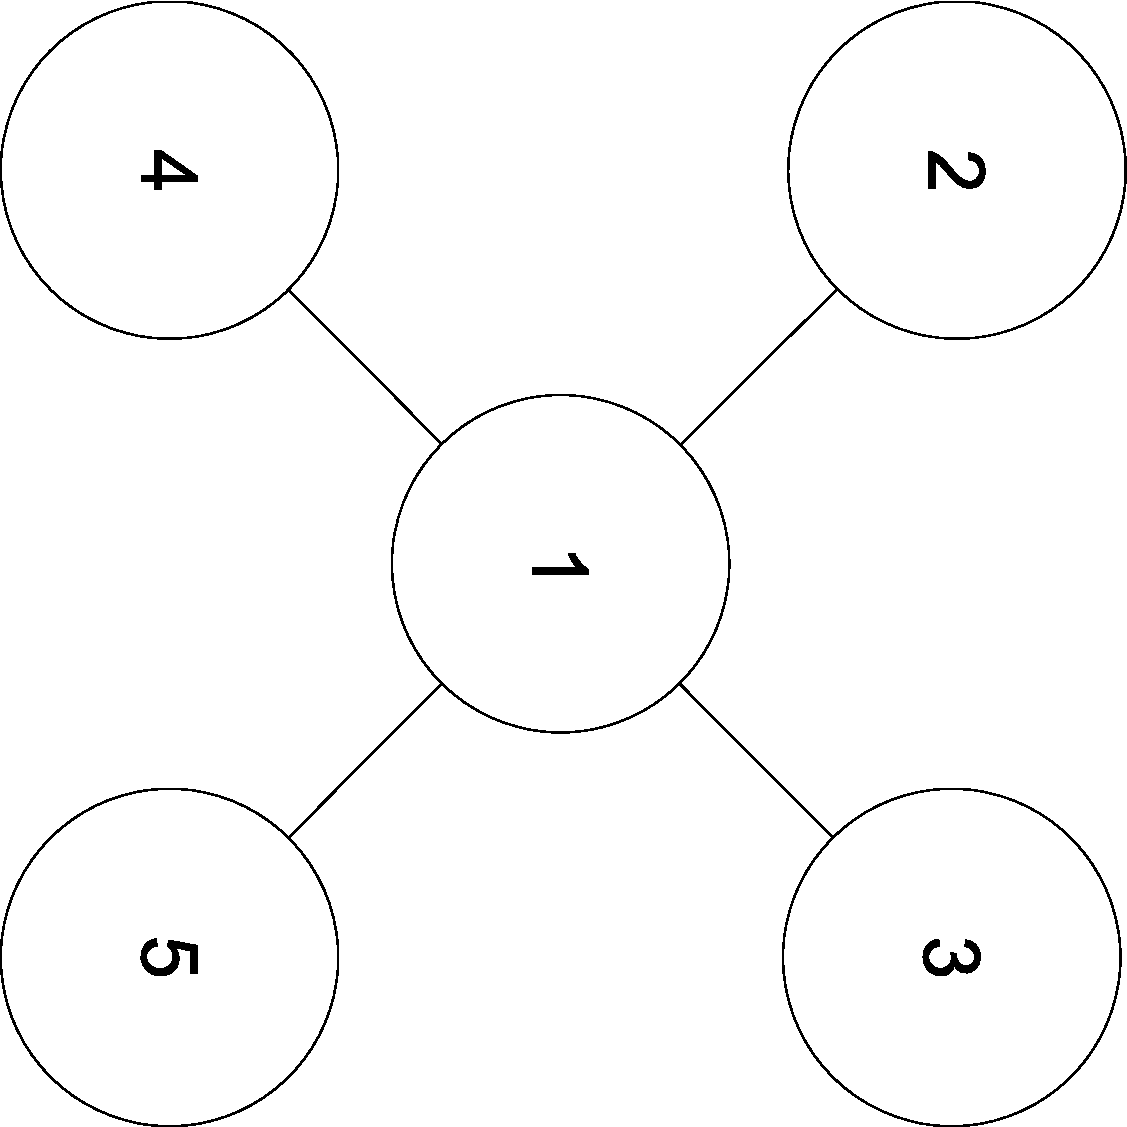
\includegraphics[angle=90,width=\linewidth]{STAR}
  \caption{A star network topology, devices are connected to a central device (in this case device 1.)}\label{fig:STAR}
\endminipage\hfill
\minipage{0.32\textwidth}
  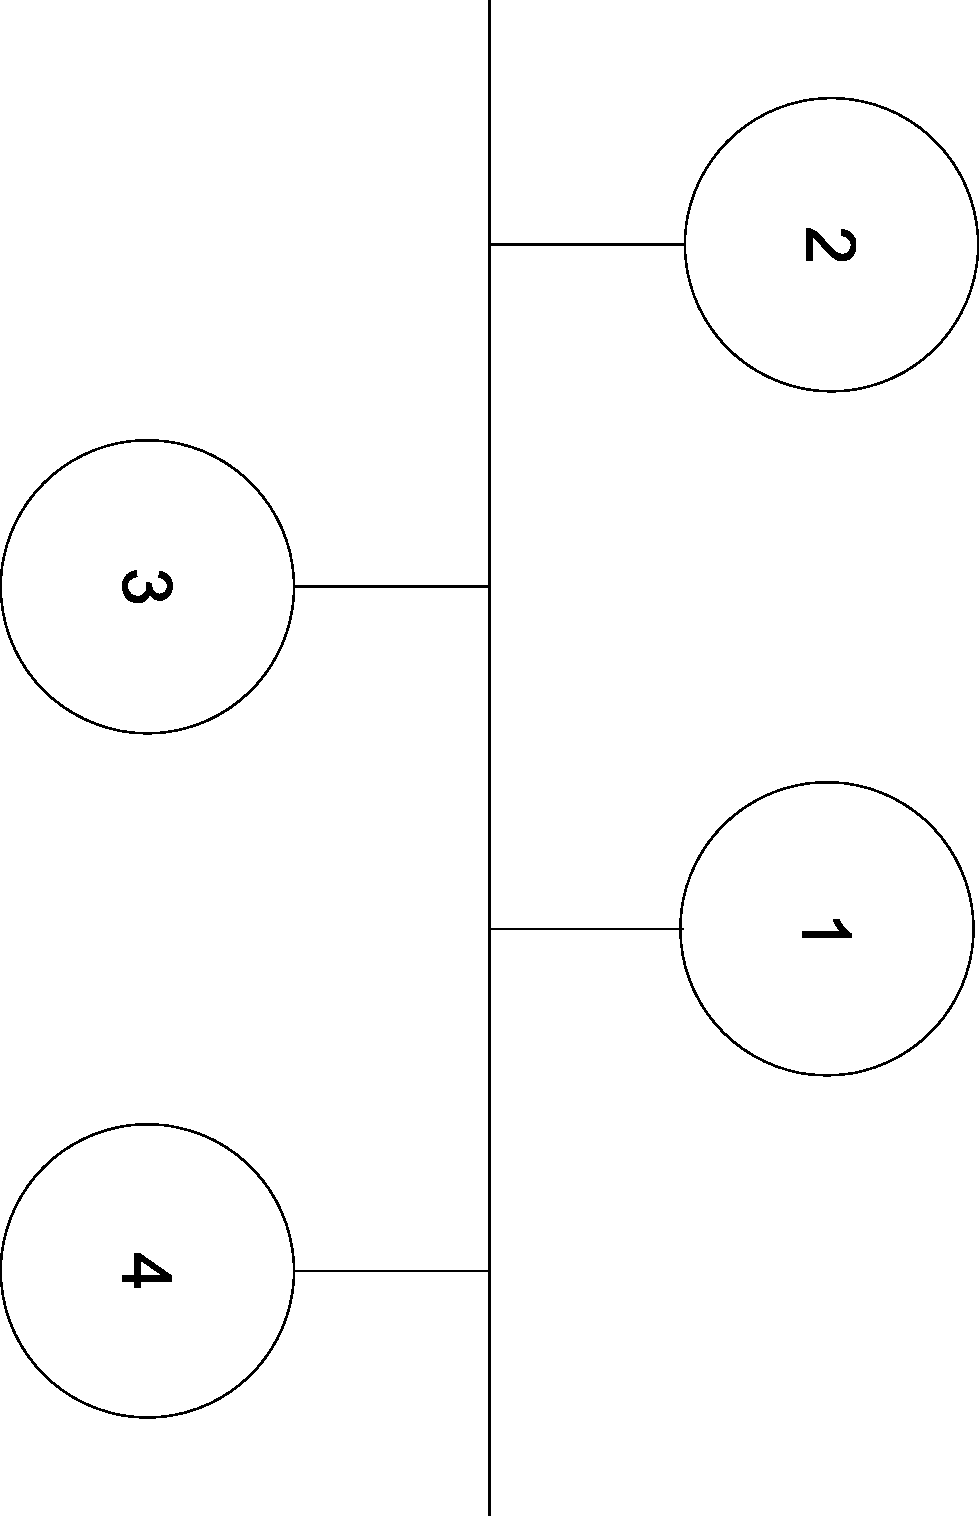
\includegraphics[angle=90,width=\linewidth]{BUS}
  \caption{A bus topology, every device is on a common link.}\label{fig:BUS}
\endminipage\hfill
\minipage{0.32\textwidth}%
  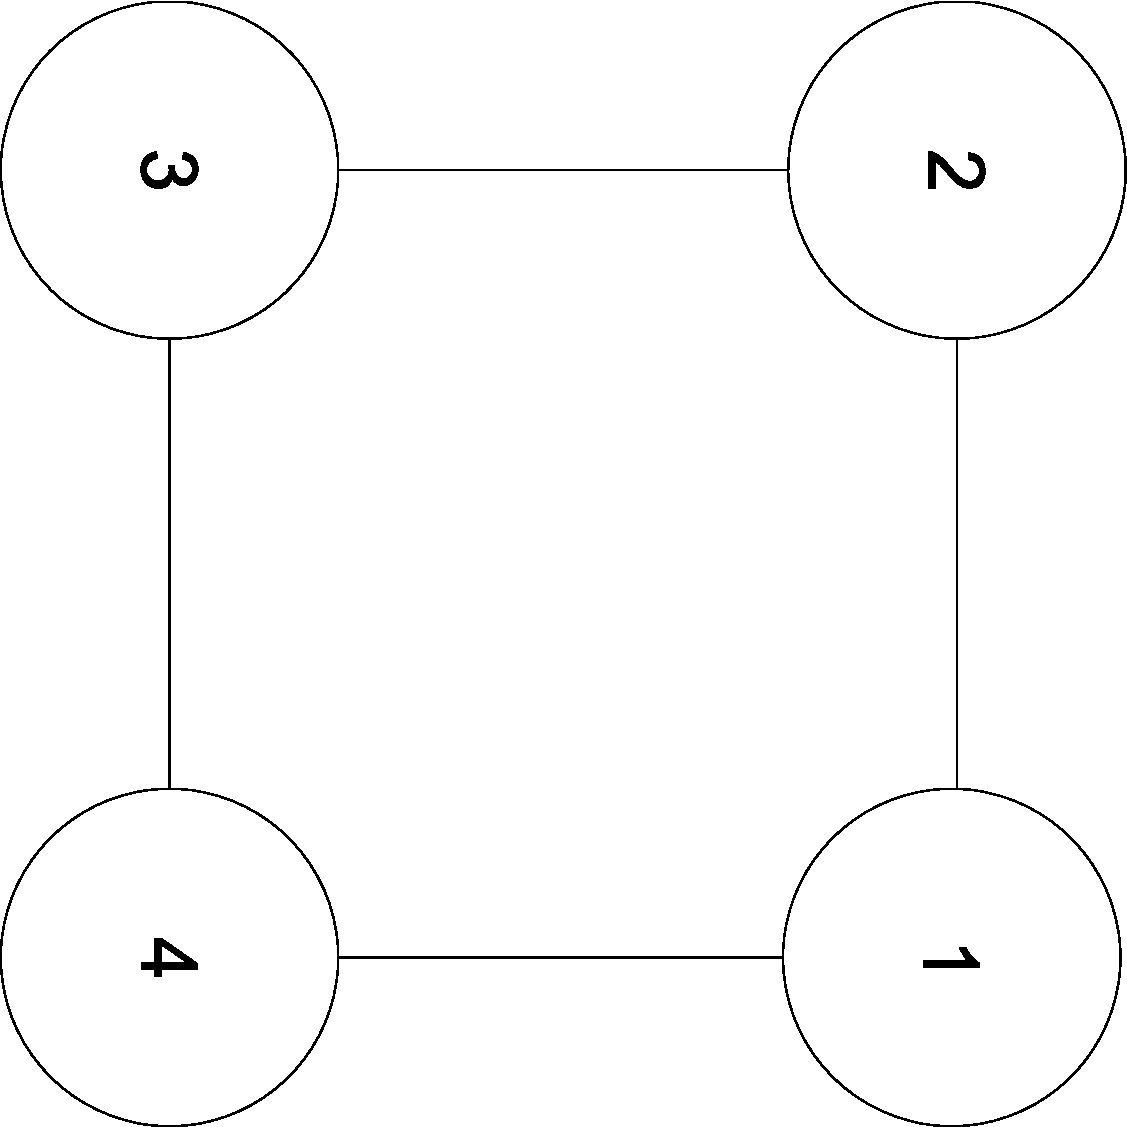
\includegraphics[angle=90,width=\linewidth]{RING}
  \caption{A ring topology, each device is connected to the next nearest device.}\label{fig:RING}
\endminipage
\end{figure}

\textbf{Star network}\\
The star network in figure \ref{fig:STAR} uses the device marked as '1' as an central switch to reach out to other devices.\cite{starwiki} When the central device fails the network will stop working. However, when one of the other nodes fail the network is not completely disabled. Because of the central device, all of the information must pass this node. This could result in speed limitations.Mainly because of the central device, the star topology is not suitable as a swarm network. \cite{combook}

\textbf{Ring network}\\
Devices in a ring network ar always connected to two other devices as displayed in figure \ref{fig:RING}. This means that there are atleast three devices in a ring network. The data distributions is unidirectional, with the traffic travelling clockwise or anticlockwise around the ring. \cite{ringwiki} This topology has it's limitations when one or more devices become isolated due to a device faillure or cable break. This problem can be solved by using a dual ring, which makes the network redundant. Because of the network topology, in which n nodes are connected serially, the communication delay is proportional to the number n devices in the network. The bandwidth is also shared between all the devices. \cite{ringwiki} It is possible to create a swarm network with a ring network but it is far from ideal.

\textbf{Bus network}\\
In a bus network the devices are connected to a linear half-duplex link. \cite{bustopology} A bus network has the advantage that it is easy to connect devices to and it works well in small networks. A disadvantage when using a bus for swarming is that the entire network shuts down when there is a break in the main connection. 
Because of this the network is not dynamic.

\textbf{Mesh network}\\
To create an network with the characteristics described in the previous section a (wireless) mesh network ((W)MN) is a possible solution. A mesh network relies on communication nodes in which data is distributed. Such a network uses multi-hopping to transport data.\cite{multi-hopwirelessnetworks} All of the communication nodes cooperate in the distribution of data in the network. Each node of the network is connected to one or more nearby in range node(s) and forwards data on behalf of the other nodes. \cite{meshnetworking} \\

There are two types of mesh networks: fully connected and partly connected mesh networks. In a fully connected network each node is directly connected to each other node in the network. This type of network is completely redundant because of the alternative connections when one of them fails. The number of needed connections can be calculated with equation \ref{eq:amountofnodes}\cite{combook}. Where 'n' is the amount of nodes and 'c' stands for the needed amount of connections. A fully connected mesh network becomes impractical when the amount of nodes increases.

\begin{equation}
c=\frac{n(n-1)}{2}
\label{eq:amountofnodes}
\end{equation}

An partly connected network is still mostly redundant, but has less connections in comparison with a fully connected network. An example of a partly connected mesh network is illustrated in figure \ref{fig:WMN}. \cite{combook} 

It is possible but not necessary to connect one or more clients of a mesh network to the internet. Thus the client connected to the internet functions as a gateway for the other clients in the network. \cite{wirelessmeshnetworksopportunitiesandchallenges}

\begin{figure}[H]
   \centering
   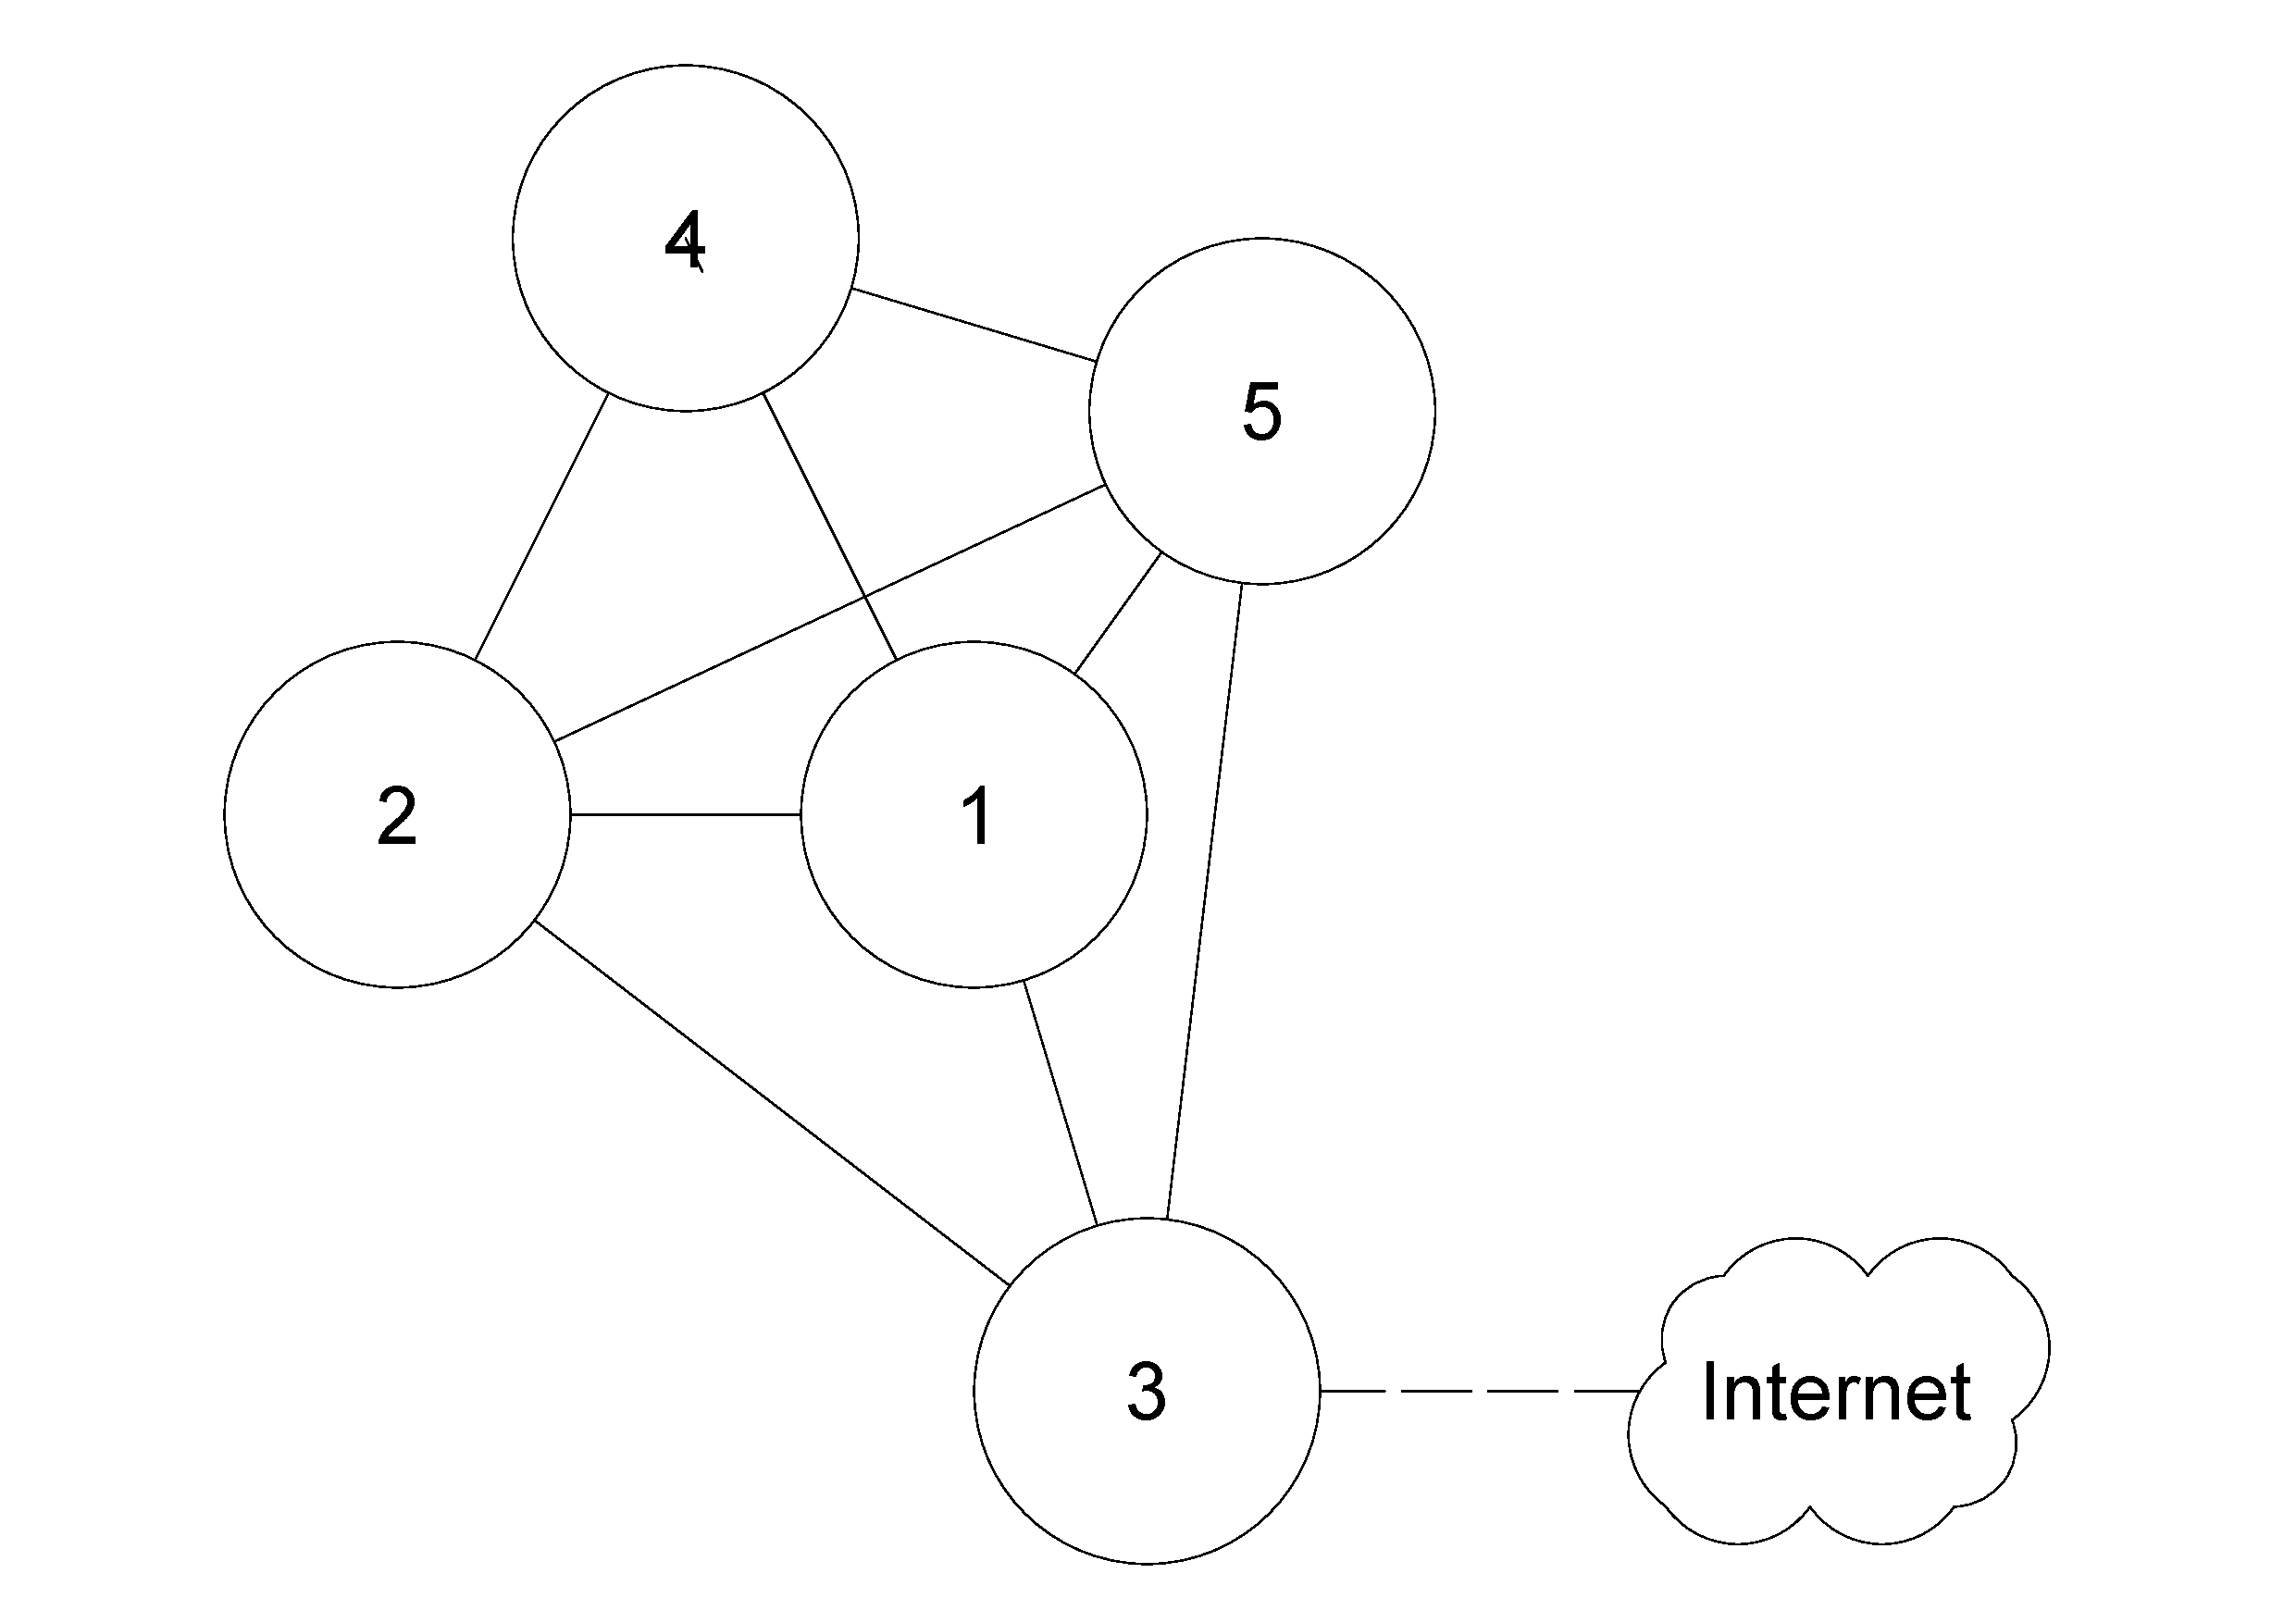
\includegraphics[width=1\textwidth]{WMN}
   \caption{An example of a wireless mesh network with 5 clients and an optional internet connection. The connections made in this example are random.}
   \label{fig:WMN}
\end{figure}

When the network topology's are compared with each other, the mesh network satisfies the desired requirements. Although it is harder to implement due to mutual connections, it has the best data coverage. To meet the given specifications, a mesh network would be the best choice.

\newpage
\subsection{Network reliability}
To ensure a realiable network, self-organization and topology control algorithms are needed.\cite{WMN1} Possibly important and usefull (wireless) network characteristics are \cite{position-based}:
\begin{itemize}
\setlength\itemsep{0em}
    \item Low construction costs
    \item Energy efficient (power aware)
    \item Cost aware
    \item Robust - Able to withstand a lost or broken client or connection
    \item Guaranteed delivery
\end{itemize}

Mesh networks can use self-healing algorithms such as Shortest Path Bridging (SPB) to restore and reroute the connection around broken nodes/clients. Shortest path bridging calculates the most favorable connections to the clients with the lowest path costs. \cite{SPB} Other usefull algorithms such as shortest path, greedy, shortest cost path, cost aware, power aware, are listed in \cite{position-based} with their characteristics. In this research only the most suitable algorithms will be discussed. 

A realiable network has a routing algorithm/protocol that includes distributed operating, loop freedom, demand-based operation and sleep period operation. Loop freedom means that the protocol is able to detect loops in the network and eliminates those. For example, data could be floating around in the network. Sleep period operating means that the clients that are not needed go into a 'sleep mode' when it's temporarily inactive.\cite{position-based}

\newpage
\subsection{Data distribution}
To set-up a reliable and stable mesh network, self-organization and topology control algorithms are needed. \cite{WMN1}\cite{position-based} This section discusses the following subjects: Data distribution strategy, routing protocols and addressing.\\

\textbf{Data distribution strategy}\\
There are several strategy's to distribute a package of data in a network. The following enumeration show three strategy's:
\begin{itemize}
\setlength\itemsep{0em}
    \item Single-path (Unicast)
    \item Multipath (Multicast)
    \item Flooding (Broadcast)
\end{itemize}

The single-path strategy is an example of the shortest path route protocol. In the single-path strategy only one packet of data in distributed in the network at a time. Which is desireable for the network capacity which is barely affected. Although the capacity is not affected, it is possible that a package is received later, because of an missing or inactive node in the path. \cite{position-based} Which results in higher latency times.

The other strategy, multipath, sends out multiple packets of data trough recognizable paths. Flooding strategy litterly floods the network with data packages. In case of wireless networks, the single-path strategy is preferred because of the power and bandwidth limitations in wireless networks. \cite{position-based}\\

\textbf{Routing protocols}\\
To meet the requirements given in the specification, the routing of the networks needs to be position based. When the position of the node in the network is known, it wil increase the networks reliability. \cite{position-based} According to the research done in \cite{geographicalrouting} and \cite{scalablelocation} routing algorithms without geographic locating (precise localization) are not scalable and won't work well in large networks.
The scalability of each algorithm means the possibility to adjust the scale of the network by adding or removing clients to the network.

There are several position-based routing protocols each with it's own characteristics a taxonomy is given in \cite{position-based}. As described earlier, only the most important protocols for the given specification will be discussed in this research. This means most of the position-based routing protocols such as: power-, cost path protocols, become irrelevant.

The shortest path route protocol uses information such as the hopcount and distance between clients to calculate the shortest route. Hopcount stands for the amount of clients that are passed by. The shortest cost path route protocol also takes account for the energy required for each routing task. The goal of this protocol is to minimize the total energy cost. According to \cite{position-based} it is not desirable or if possible to avoid to memorize routes or past traffic in mobile ad hoc networks. This is because of the mobility of clients in the network and constantly changing infrastructure.

The distance between neighboring nodes can be estimated on the basis of signal strengths or time delays in direct communications. The exact positions can for example be estimated by using positioning systems such as GPS (Gereral positioning system). \cite{locationsystemsforubiquitouscomputing} The approximation of the position of the node relative to the other nodes can be done by several methods.

In figure \ref{fig:greedyrouting} a greedy routing scheme is displayed. The node S contains the data package and D is the destination of the package. 

\begin{figure}[H]
   \centering
   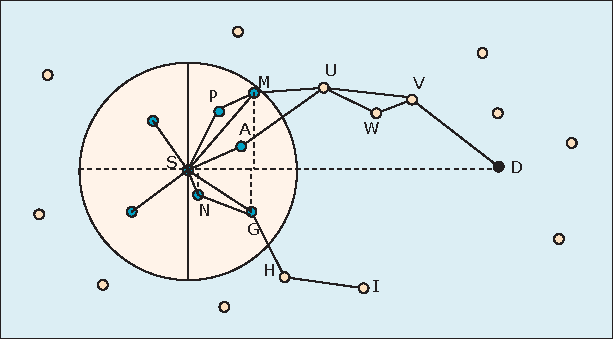
\includegraphics[width=1\textwidth]{greedyrouting}
   \caption{Greedy round scheme found in \cite{position-based}. "S selects M in MFR path SMUVD, G in greedy path SGHI that
fails to deliver, A in direction-based-path SAUWVD, P in power path
SPMUWVD, N in NFP/NC path SNGHI that fails to deliver."}
   \label{fig:greedyrouting}
\end{figure}

The principle of greedy routing is that it is trying to get closer to the destination based on local information. Thus the data package is forwarded to the client/node which is the most suitable from a local point of view. \cite{geographicrouting} "Greedy schemes have a performance close to performance of optimal shortest path (weighted) algorithm for dense graphs, but have low delivery rates for sparse graphs. Schemes that guarantee delivery may have high communication overhead for sparse graphs." \cite{position-based}\cite{positionbasedroutingtaxonomy} \\

The most efficient algorithm for path bridging depends on the situation where the clients are operating in which is described in \cite{position-based}\cite{positionbasedroutingtaxonomy}. As stated earlier, in this stage of the development some characteristics are irrelevant, the energy efficient and cost routing protocols for example. There are however some characteristics that do matter. The single path strategy for example, is preferred because of bandwidth limitations in wireless networks. It is also not preferred to memorize the routes of past traffic in mobile networks.\cite{position-based} \cite{positionbasedroutingtaxonomy} Given these characteristics, the most suitable method will be greedy routing or a derivative/improved version.


\textbf{Addressing}\\
Each node in a mesh network needs a address for other nodes to refer to. Methods to address meshed networks are:
\begin{itemize}
\setlength\itemsep{0em}
    \item Adaptive robust tree (ART)
    \item Meshed adaptive robust tree (MART)
\end{itemize}
Most of the wireless network protocols already cover the dressing in the protocol itself. The following methods are a possible compliment.

\textbf{Adaptive robust tree (ART)}\\
Adaptive robust tree is a meshed tree routing approach to address the nodes. Each node is adaptively addressed during the tree formation. It is desirable that the tree is free of single point failures (SPOF). This means that there is always a redundant path if a node fails, but that's not always possible in non-mesh networks. Each node keeps track of an ART table (ARTT), to map it's branches. In this table the addresses of the connected branches are stored.

ART knows three phases; the initialization, operation and recovery phase. In the initialization phase the tree is formed. The tree formation starts at the root and grows by adding nodes to the tree. The nodes get an address assigned, when all nodes are joined. Thereafter, the number of nodes are counted in the tree as shown in figure \ref{fig:treenumbers}.


\begin{figure}[H]
   \centering
   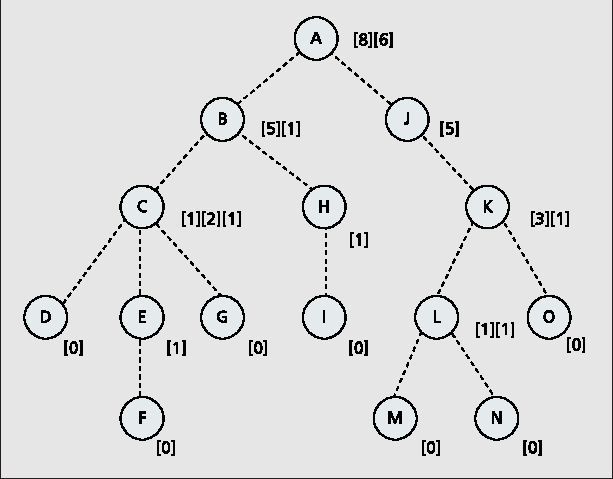
\includegraphics[width=1\textwidth]{treenumbers}
   \caption{An example of a wireless mesh network with 5 clients and an optional internet connection. The connections made in this example are random.}
   \label{fig:treenumbers}
\end{figure}

The following phase is the operation phase, where small amount of nodes are still able to join, but when the change becomes to big, the network goes in to initialization mode again. When a part of the tree becomes broken, the recovery phase becomes active for the affected part.\\

\textbf{Meshed adaptive robust tree}\\
With an ART tree it is possible to create a MART (Meshed adaptive robust tree). Figure \ref{fig:meshtree} illustrates a MART, in this figure there are already connections added that make a mesh network. The intermittent lines are added for the mesh network. From the point of view from every node in the network, there still is a tree form. In this mesh network, each node has a redundant path if a connection is broken, so it is SPOF free.

\begin{figure}[H]
   \centering
   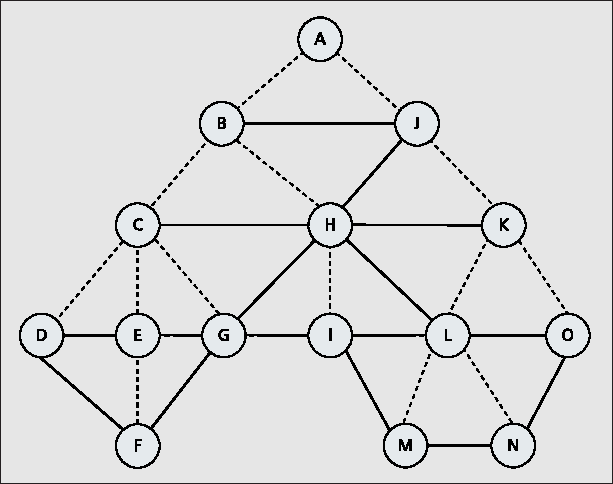
\includegraphics[width=1\textwidth]{meshtree}
   \caption{Meshed ART formation based on figure from \cite{emergingstandarsforwirelessmeshtechnology}}
   \label{fig:meshtree}
\end{figure}

With a MART, it is possible to reroute a connection to reduce the path cost in comparison with ART. Most of the time, the transition from ART to MART, removes some SPOFs.

\subsection{Wireless mesh network}
A mesh network (MN) is a dynamically self-organized and configured network. \cite{WMN1} As described in the specifications, the swarm network is dynamic in size and mutual distance. Because of the size and mobility of the swarm it is not practical to use wired connections between de members of the swarm. So a wireless mesh network (WMN) is needed. Therefore a wireless connection between the members is necessary.

Despite the practical benefits of wireless networks, today's wireless networks still cannot offer the same level of sustained bandwith as their wired brethren. The bandwidth is for instance affected by interference from adjacent hops on the same and neighboring paths. \cite{architectureandalgorithmsmultichannelwirelessmeshnetwork} One of the most important drawbacks is that each client needs to be in transmitting and receiving range to atleast one of the other clients to be connected to the network. \cite{wirelessmeshnetworksopportunitiesandchallenges} Another con is that the data rate falls quickly when increasing the distance between transmitter and receiver, which doesn't or barely apply to wired networks. \cite{architectureandalgorithmsmultichannelwirelessmeshnetwork} The complexity of an WMN network is also a main drawback. It is relatively easy to design a WMN, but it is difficult to achieve an optimum performance while ensuring security and robustness.\cite{wirelessmeshnetworksopportunitiesandchallenges} 

Each node or client in the network is able to create an ad hoc network to maintain the mesh connectivity, this is called "client WMN's". These networks are able to reroute around nodes that have been lost. On large scale projects wireless mesh networks are costefficient because of the saving of wired connections.\cite{meshnetworking} 

Nevertheless, the client mobility weigh out the cons described earlier. So solutions must be found to overcome these drawbacks.

\newpage
\subsection{Wireless network protocols}
As stated earlier, the communication in the network needs to be wireless. This makes the network flexible in scaling, gives the nodes full freedom of movement and saves physical connections which could be cost efficient.

The following wireless protocols or technologys are defined as short-range (a range of 10-100m) communication protocols \cite{emergingstandarsforwirelessmeshtechnology} \cite{combook}:
\begin{itemize}
\setlength\itemsep{0em}
    \item IEEE 802.11 a/b/g/ac/s (Wi-Fi) \cite{IEEE80211timeline}
    \item IEEE 802.15.1 (Bluetooth)
    \item IEEE 802.15.4/5 (ZigBee)
    \item IEEE 802.15.3 (Ultra-wideband)
    \item IR IrDA(Infrared)
\end{itemize}
 There are however exceptions, some of the technology's have been evolved and are able to transmit further than 100 meters. WiMax for example is developed to overcome the range problem. 
\begin{itemize}
\setlength\itemsep{0em}
     \item IEEE 802.16 (a) (WiMAX)
\end{itemize}

\paragraph{IEEE 802.15.1 Bluetooth}
Bluetooth is designed for short-range communication which uses wireless radio systems. Bluetooth is mostly used for personal-area networks (PAN). \cite{combook} The main purpose of Bluetooth is to create a wireless connection between for example computer peripherals such as; keyboards and mice. These applications are also known as wireless personal area networks (WPAN). \cite{comparitivestudywirelessprotocols} Bluetooth is an ad hoc network, which means that the network is formed spontaneously.\cite{tcipbook}

Bluetooth uses the industrial scientific and medical (or short: ISM) band for receiving en transmission data. The ISM band ranges from 2,400 to 2,4835 GHz in the Netherlands. \cite{frequencyandsnetherlands} Frequency hopping spread spectrum (FHSS) is used to spread out the power over the full bandwidth. After the transmission of each packet, Bluetooth will hop/change to another channel. The ISM band consists of 79 channels with 1 MHz each. Changing frequencies also helps to avoid collision with other networks. But it is still possible that a collision takes place. When a collision happens, the data is resend on another channel until the transmission is successful.

\begin{figure}[H]
   \centering
   \includegraphics[width=1\textwidth]{Bluetoothfh}
   \caption{Bluetooth frequency hopping spread spectrum (FHSS) from \cite{Bluetoothspectrum}}
   \label{fig:Bluetoothfh}
\end{figure}

Bluetooth consists of two network topologies: a piconet and scatternet. The piconet has one or more slaves serving one master \cite{Bluetoothpiconet}. In a piconet the master synchronizes the master's clock and shares his Bluetooth device address at the first connection. The data packet is called a frequency-hopsynchronization packet (FHS packet). The data send in the FHS packet is used to calculate the sequence of frequency hops that all devices in the piconet will follow. Each client in the networks tracks the native- and masters clock, so it will know on which frequency the client needs to transmit or receive.

Each piconet has one master which has an unique Bluetooth device adress and clock. A Bluetooth piconet cannot be large. A piconet consists of 8 active clients in which one is the 'primary' (master).\cite{tcipbook} There can be 255 slaves in a parkmode in a Bluetooth piconet. Because of the frequency hopping, it is possible to have more than one piconets in one area. 

A scatternet consists of two or more piconets. It is possible for a client to participate in more than one piconets, but it can only be a master of one network. Figure \ref{fig:scatternet} illustrates a complex scatternet.

\begin{figure}[H]
   \centering
   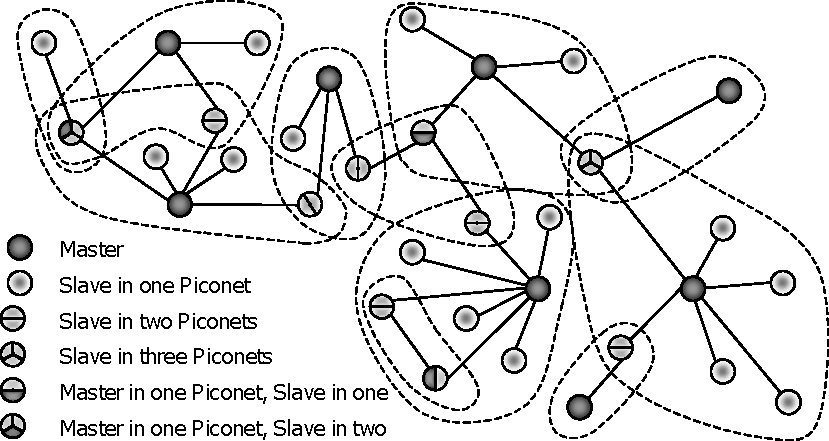
\includegraphics[width=1\textwidth]{scatternet}
   \caption{A complex scatternet found in \cite{Bluetoothwifisurveyandcomparison}}
   \label{fig:scatternet}
\end{figure}

The biggest drawback by using Bluetooth is that it doesn't officially support mesh networking. According to the IEEE timeline \cite{IEEE80211timeline}, there will be a mesh standard for Bluetooth in the year 2016. \cite{Bluetoothmesh} At the time of this research (begin 2016), the standard is not published yet neither, are there implementation available. It is still possible to create a scatternet, with multiple masters/slaves but that doesn't meet the given specifications. \\

\paragraph{IEEE 802.15.4 ZigBee}
Zigbee is usually used in personal operating spaces (POS) or personal-area networks (PAN) of about 10 meters. \cite{combook} However, there are devices based on Zigbee that can reach up to 1500 meters of span when the target is in line of sight \cite{zigbeewiki}. It is designed for simple devices that consume minimal power and operate in a personal operating space. Applications as sensors. These applications are also known as low-rate wireless personal area networks (LR-WPAN). \cite{comparitivestudywirelessprotocols} Zigbee uses the ISM 900 MHz or, just like Bluetooth and WiFi, the 2,4 GHz ISM band to communicate. Zigbee uses direct sequence spread spectrum (DSSS) with 16 channels and 2 MHz bandwidth.

There are proven implementations of networks with ZigBee. It is possible to create a reliable self-organized mesh network which is able to use multi-hopping \cite{comparitivestudywirelessprotocols}.

Zigbee is known for the low power consumption which results in long battery lifetime \cite{performanceevaluationlowratewirelesspan}. There are two types of devices in a LR-WPAN network: A full-functioning device and a reduced-functioning device. Full-functioning devices can be used as a 'Master' or coordinator or as a client. These devices can talk to each other, or to reduced-functioning devices. A RFD is used for simple transmit tasks such as switches or simple in/output operations. Just like Bluetooth, the coordinator or master, will set the network up.

Zigbee supports multiple network topology's such as: Star, tree and mesh networks. This means that it is compatible to work with mesh networks. \cite{zigbeewiki}


\paragraph{IEEE 802.11 Wi-Fi}
Wireless local area networks (WLANs) or IEEE 802.11 is popularly known as Wi-Fi (Wireless Fidelity) \cite{wirelessmeshnetworksopportunitiesandchallenges}. With a Wi-Fi connection it is possible for the clients to connect to the internet with broadband speeds. Consumer WiFi usually uses one or two ISM frequency bands: 2,4 and 5 GHz. The 2,4 GHz unlicenced ISM band used for IEEE 802.11b/g/n/s extends from 2.4 to 2,4835 GHz with a total bandwidth of 83.5MHz. The 5 GHz ISM band used for IEEE 802.11a extends from 5.15 to 5.25 GHz with a power limitation of 50mW, 5.25 to 5.35 Ghz with 250mW and5.725 to 5.825 GHz with 1W of power.\cite{combook} The benefit of using the 5 GHz ISM band is that there are alot less interference from appliances like microwaves, Bluetooth products and a number of other services. The downside of 5 GHz is however, the transmission range decreases greatly because 5 GHz signals are absorbed faster in comparison with 2,4 GHz signals. \cite{combook} There are also Wi-Fi standards which use the 3,6 and 60 GHz band. The 3,6 GHz band is used by the IEEE 802.11y-2008 standard and the 60 GHz band for the IEEE 802.11ad protocol. The 802.11 standard defines two services: the basic set (BSS) and the extended service set (ESS). The basic service set without an acces point is an ad hoc network and only consists of accespoints. All devices in a BSS use the same channel.\cite{Bluetoothwifisurveyandcomparison}

Wi-Fi uses different modulation techniques. Direct sequence spread spectrum (DSSS), Orthogonal frequency division multiplexing (OFDM) and code keying (CDK) with 14 possible channels on the 2,4 GHz band. With DSSS it is possible that multiple signals use the same channel. However to prevent interference the channel selection must be criticially considered. Each channel has a bandwidth of 22 MHz and is 5MHz apart, see figure \ref{fig:wifichannels}. \cite{combook} Because of the span of each channel, the channels overlap.

\begin{figure}[H]
   \centering
   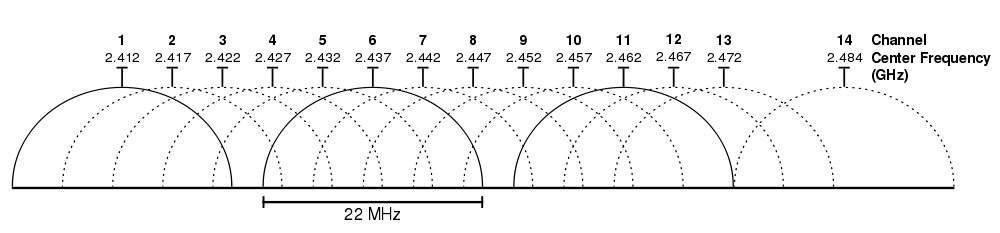
\includegraphics[width=1\textwidth]{wifichannels}
   \caption{Illustration of the Wi-Fi channels on the 2,4 GHz band. \cite{wifichannels}}
   \label{fig:wifichannels}
\end{figure}

Wi-Fi doesn't use frequency hopping to avoid data collisions. This forms a problem when there are hidden nodes in the network. A hidden node is illustrated in figure \ref{fig:hiddennode}. The circles indicate the transmission range of each node. In figure \ref{fig:hiddennode} 'A' is not in the transmission range of 'C', which makes 'A' invisible to 'C'. In this situation node A and C are not aware of each other. Therefore one of the nodes can think that it is the only active node in the network.

\begin{figure}[H]
   \centering
   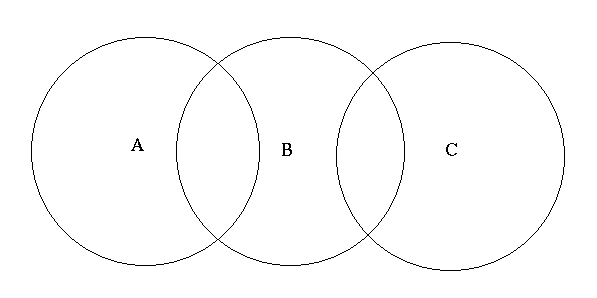
\includegraphics[width=1\textwidth]{hiddennodeproblem}
   \caption{Illustrates the hidden node problem with three nodes.}
   \label{fig:hiddennode}
\end{figure}

In the following situation there will be a collision of information:
\begin{itemize}
\setlength\itemsep{0em}
\item Node 'A' sends data to node 'B'.
\item Simultaneously node 'C' is also sending information to node 'B'.
\end{itemize}

Using handshake frames (CSMA/CD - CA) can be a solution to prevent a collision from happening when there is a hidden node. With 802.11, the used handshakes frames are CTS (clear to send) and RTS (request to send). The solution is given in figure \ref{fig:rtscts}. Where node 'A' send an RTS to 'B' and 'B' responds with an CTS to node 'A' and 'C'. Node 'C' didn't send an RTS, so the node knows that it needs to wait. The waiting duration of data transmission is contained in the CTS message which is send by node 'B'. \cite{tcipbook}

\begin{figure}[H]
   \centering
   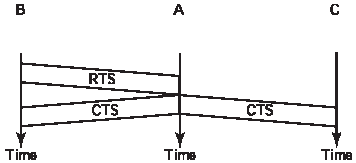
\includegraphics[width=.75\textwidth]{rtscts}
   \caption{Gives an example of the hidden node problem given in \ref{fig:hiddennode}}
   \label{fig:rtscts}
\end{figure}

As mentioned before, using handshake frames can be a solution to prevent a data collision from happening in case of a hidden node. However, in a exposed node problem, this method will cause data transmission inefficiency. \cite{tcipbook} Figure \ref{fig:exposedstation} illustrates the exposed node problem. In figure \ref{fig:rtscts2} the following situation is illustrated:

\begin{itemize}
\setlength\itemsep{0em}
\item Node 'A' wants to send information to the node 'B'.
\item Node 'C' also wants to send information to node 'D'.
\item Because node 'C' receives an RTS, it doesn't get permission to send an RTS itself.
\end{itemize}

\begin{figure}[H]
   \centering
   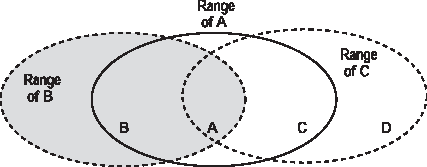
\includegraphics[width=1\textwidth]{exposedstation}
   \caption{The exposed node problem with four nodes and two nodes who want to send information.}
   \label{fig:exposedstation}
\end{figure}

\begin{figure}[H]
   \centering
   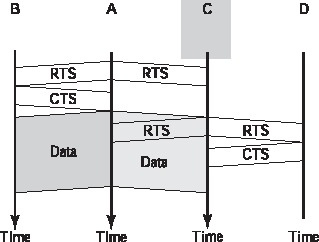
\includegraphics[width=.75\textwidth]{rtscts2}
   \caption{Gives an example of the exposed node problem given in \ref{fig:exposedstation}}
   \label{fig:rtscts2}
\end{figure}

To prevent these problems, frequency- or channelhopping is a solution. \cite{architectureandalgorithmsmultichannelwirelessmeshnetwork} has done research in multi-channel wireless mesh networks and have proven that it is practically possible.

IEEE 802.11s is a Wi-Fi standard for mesh networking. This standard defines how stations can interconnect to form a mesh network. Many other implementations of 802.11 do not interconnect the base stations with eachother and this standard does. \cite{ieee80211sthewlanmeshstandard}

The 802.11s standard defines a mandatory default scheme for path selection. This default scheme can be replaced by other path selection protocol because of the extensible framework of the standard. By default the Hybrid Wireless Mesh Protocol (HWMP) is used as a path selectiong protocol. HWMP is derived from the Ad Hoc On Demand Distance vector (AODV) protocol. \cite{ieee80211sthewlanmeshstandard}

Open80211s is an implementation of the 802.11s standard. According to \cite{ieee80211sthewlanmeshstandard} this standard will be able to run on legacy 802.11 cards with software adjustments. Figure \ref{fig:open80211s} gives an impression of the network performance in a 12 node dense network. 
\begin{figure}[H]
   \centering
   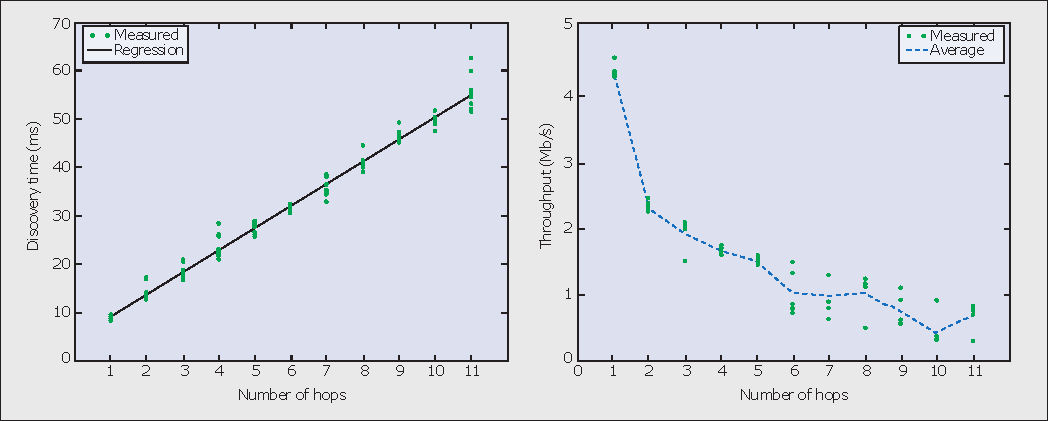
\includegraphics[width=1\textwidth]{open80211s}
   \caption{\cite{ieee80211sthewlanmeshstandard} gives an performance measurement of the open80211s implementation in 2010.}
   \label{fig:open80211s}
\end{figure}
As shown in figure \ref{fig:open80211s}, the discovery time increases linearly with an increasing number of node hops. This decreases the throughput of the network.

\paragraph{IEEE 802.15.3 Ultra-wideband}
Ultra-wideband is designed for short-range high-speed wireless communication. The bandwidth of UWB is over 100Mbps and can reach speeds up to 480 Mbps \cite{comparitivestudywirelessprotocols}. UWB is a high data rate Wireless Personal Area Networks (HR-WPAN). The frequency band of UWB ranges from 3.1 to 10.6 GHz \cite{ultrawidebandwirelesscommunications}. Although the spectrum is large in comparison with other protocols the signal level is very low so it doesn't interfere with other signals. UWB is a baseband or carrierless communication method. These systems use precisely timed impulses to transmit data on the wide spectrum. This divers from other communication methods where sine modulation is used. \cite{Bluetoothwifisurveyandcomparison}

Because of the 'ultra wide' band UWB has benefits over other technologys. The benefits of UWB are \cite{ultrawidebandwirelesscommunications}\cite{combook}: 
\begin{itemize}
\setlength\itemsep{0em}
    \item High data rates
    \item Less path loss and better immunity to multipath propagation
    \item Low-cost transceivers
    \item Low transmit power and low interference
\end{itemize}
 With UWB it is possible to get high data rates in ranges of 20 to 50 meters. Because of the wide bandwidth of UWB, the material penetration losses are relatively low. As shown in equation \ref{eq:channelcapacity}, the channelcapicity increases linearly with the bandwidth.

 \begin{equation}
    C=Blog_2(1+\frac{S}{N})
    \label{eq:channelcapacity}
 \end{equation}

 Because of the absence of sending a carrier, the transceiver build can be relatively simple. \cite{ultrawidebandwirelesscommunications} The disadvantage is however, the transmitpower must be low for commerical use. This results in a low transmitting range about 30 meters according to \cite{combook}.

UWB devices are like Bluetooth devices organised in piconets. Each piconet is controlled by a dedicated coordinator (PNC). The benefit of using UWB is however that each devices can communicate in peer to peer with an other device in contrast to Bluetooth. When the devices are not in range of eachother, the coordinators work as an intermediary to connect device 'A' to 'B'. Mesh networks topology's are supported, but it will be using bridges between piconets to maintain the network. Like Wi-Fi UWB also uses a form of CSMA-CA when there are devices competing for acces. \cite{piconetinterconnectionstrategies}

\paragraph{IR Infrared}
Infrared is possibly the most widespread wireless technology for short-distance data communication. \cite{combook} It is primarily used for remote control between computers and televisions. The short-range distance with infrared communications is typically about 1 to 9 meters. \cite{combook} Infrared travels with the speed of light which is 299792458 meters per second. \cite{speedoflight} In comparison with the other discussed protocols this technology is based on light instead of radio frequency signals. Because of the origin of this technology, there must be a clear (no obstacles block the sight) line of sight (LOS) between the transmitter and receiver. This disadvantage makes the technology not suitable for the communication in a complex swarm network.\\

\paragraph{IEEE 802.16 WiMAX}
WiMAX in the United States or HIPERMAN in europe is a wireless metropolitan-area network (MAN network). \cite{draadlozecommunicatie} WiMAX is defined by the IEEE 802.16 standard. The main reason for developing this standard was to deliver consumers wireless broadband speeds. WiMAX networks are managed by network operators.

WiMAX is a long-distance data communication technology. The maximum theoretical distance reached by this protocol is defined as 50 km. The used frequency band ranges from 2 to 11 and 10 to 66 GHz with the 802.16(a) standard. The higher frequency range is only used for line of sight (LOS) transmission and the lower range for (NLOS) not line of sight transmission.\cite{draadlozecommunicatie}

WiMAX knows three topology structures: Point-to-point (P2P), point-to-multipoint (PMP) and mesh mode. \cite{combook}

To realise the high transmit ranges, high transmit power is needed. A typical basestation consumes approximately 20W and the mobile stations 200mW. A mobile station can easily receive the transmission from a basestation. The communication from the mobile station to the basestation however is more difficult to receive, because of the low transmitting power.
\cite{wimax}

In comparison with Wi-Fi, WiMAX is more based on the master-slave technique. The basestation has complete control over the transmission. This characteristic and the high power usage makes and the dependence on a network provider makes this protocol does not meet the criteria for the described swarm network.\\

\paragraph{General comparison}
To summarize the given information from the protocols, table \ref{sumtableprotocols} is made. This table displays the most important characteristics of each protocol.

\begin{table}[H]
\centering
\caption{A table with a summerazing of the protocols. The table is based on information from \cite{comparitivestudywirelessprotocols}. Infrared is not included due to the line of sight problem.}
\label{sumtableprotocols}
\resizebox{\textwidth}{!}{\begin{tabular}{|l|l|l|l|l|}
\hline
\textbf{Standard}        & \textbf{Bluetooth} & \textbf{Ultra-wide band} & \textbf{ZigBee}      & \textbf{Wi-Fi} \\ \hline
IEEE spec.               & 802.15.1           & 802.15.3a                & 802.15.4             & 802.11a/b/g    \\ \hline
Frequency band           & 2.4 GHz            & 3.1-10.6 GHz             & 868/915 MHz; 2,4 GHz & 2,4GHz; 5GHz   \\ \hline
Max signal rate          & 1Mb/s              & 110Mb/s                  & 250Kb/s              & 54Mb/s         \\ \hline
Nominal range            & 10m                & 10m                      & 10-100m              & 100m           \\ \hline
Channel bandwidth        & 1 MHz              & 500 MHz - 7.5 GHz        & 0.3/0.6 MHz; 2MHz    & 22 MHz         \\ \hline
Basic cell               & Piconet            & Piconet                  & Star                 & BSS            \\ \hline
Extension basic cell     & Scatternet         & Peer-to-peer, mesh            & Cluster tree, mesh   & ESS, mesh            \\ \hline
Max cell nodes & 8  \cite{combook}                & 8                        & \textgreater65000\cite{combook}    & 2007           \\ \hline
\end{tabular}}
\end{table}

Each characteristic of the protocol is compared with each other in this chapter. And for each comparison the most suitable and unsuitable characteristic is given pros and cons. This way a recommendation can be made.\\

\textbf{Network size}\\
The networkssize of each of the protocols is expendable. This is shown in table \ref{sumtableprotocols}. A Bluetooth piconet for example can be part of a scatternet, which overlooks serveral other piconets. However, each piconet must have a master as mentioned before, a master in a swarm network is not desirable. Bluetooth also doesn't have mesh network support yet (begin 2016). \cite{bluetoothmesh} This gives Bluetooth the biggest disadvantage in contrast to the other protocols. In comparison with ZigBee which has the biggest possible network size.\\


\textbf{Transmission time}\\
The transmission latency between nodes can be calculated with equation \ref{eq:transmissiontime}.\cite{comparitivestudywirelessprotocols} The data size ($N_{data}$), the maximum payload size ($N_{maxPld}$), the overhead size ($N_{ovhd}$), the bit time ($T_{bit}$) and the propagation time ($T_{prop}$) between devices form the transmission latency ($T_{tx}$). 

\begin{equation}
    T_{tx}=(N_{data} + \Bigg(\frac{N_{data}}{N_{maxPld}} N_{ovhd} \Bigg) T_{bit} + T_{prop})
    \label{eq:transmissiontime}
\end{equation}

When the data payload size increases the transmission time increases as shown in \cite{comparitivestudywirelessprotocols}. In comparison to the other protocols, UWB has the lowest bit time which results in the fastest transmission time followed by Wi-Fi. Where ZigBee followed by Bluetooth have the slowest transmission time.

As mentioned earlier, the density of a Wi-Fi network, contributes to the network latency due to the exposed node problem.\cite{combook} \\

\textbf{Data distribution per square meter}\\
Research done in \cite{ultrawidebandshortmediumrange} makes a data distribution comparison between Wi-Fi, Bluetooth and Ultra-wideband. Because of the crowding in the spectrum and the growing demand for wireless data capability at high bandwidth it favors systems just not to have a high-peak bit rate, but also high spatial capacity. Spatial capacity is defined as bits/sec/square-meter. \cite{ultrawidebandshortmediumrange} Table \ref{spatialcapacity} gives the spatial capacity of each protocol.

\begin{table}[H]
\centering
\caption{Spatial capacity of different protocols, based on information from \cite{ultrawidebandshortmediumrange}}
\label{spatialcapacity}
\begin{tabular}{|l|l|}
\hline
\textbf{Protocol}  & \textbf{Spatial capacity} \\ \hline
Wi-Fi IEEE 802.11b & 1.000                     \\ \hline
Wi-Fi IEEE 802.11a & 83.000                    \\ \hline
Bluetooth IEEE 802.15.4          & 30.000                    \\ \hline
UWB IEEE 802.15.3a                & 1.000.000                 \\ \hline
\end{tabular}
\end{table}

\begin{figure}[H]
   \centering
   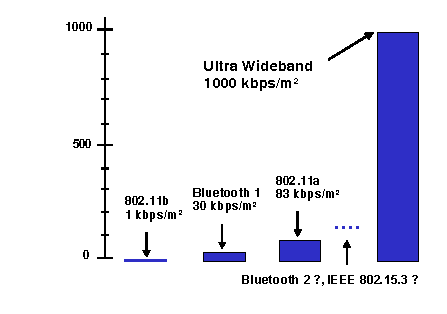
\includegraphics[width=1\textwidth]{spatialcapacity}
   \caption{Comparision of the spatial capacity for each protocol, found in \cite{ultrawidebandshortmediumrange}.}
   \label{fig:protocolcomplexity}
\end{figure}

\textbf{\\Protocol complexity}\\
The protocol complexity can be compared by the number of primitives and events in a set situation. When there are more primitives or events in a certain protocol, it indicates the complexity. \cite{comparitivestudywirelessprotocols} As indicated in figure \ref{fig:protocolcomplexity} Bluetooth is by far the most complex protocol compared to the other protocols.

\begin{figure}[H]
   \centering
   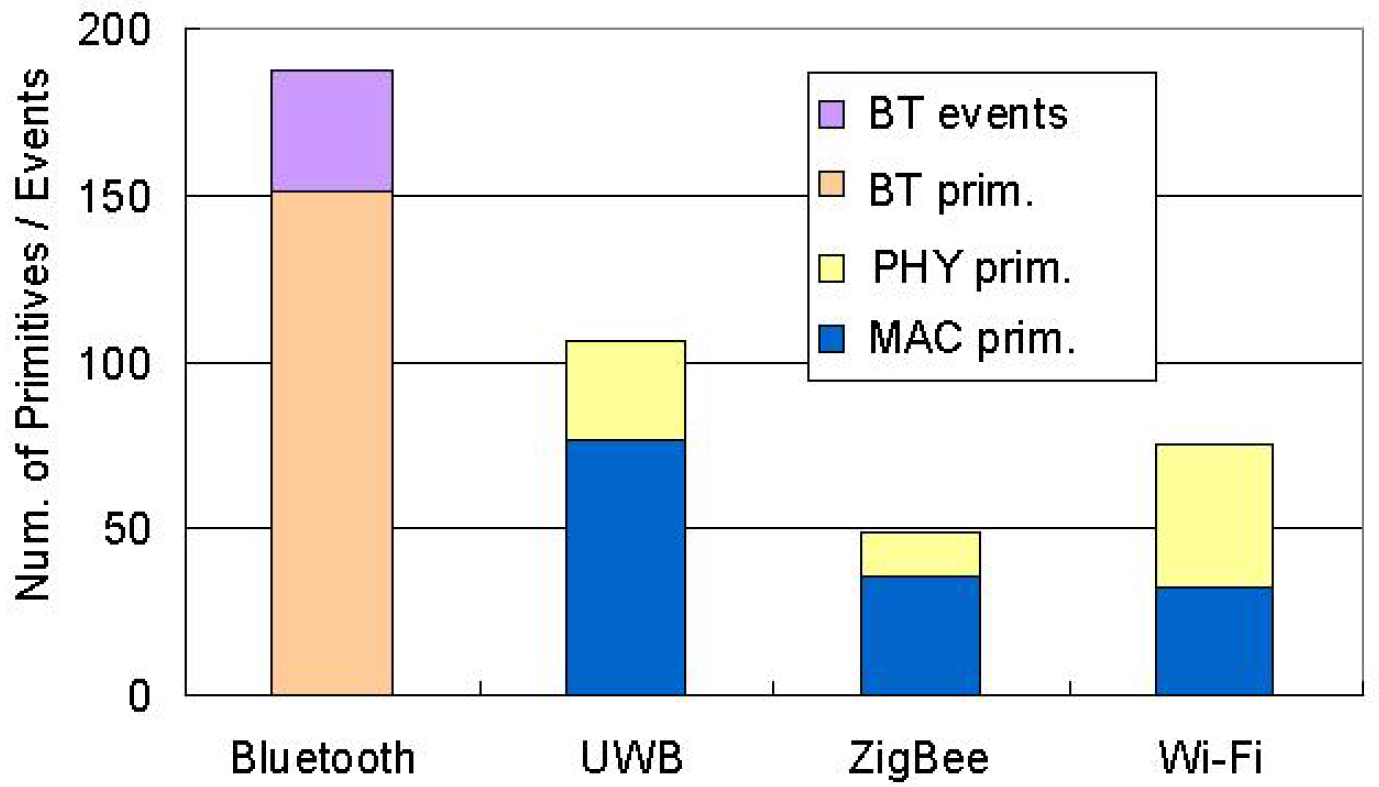
\includegraphics[width=1\textwidth]{protocolcomplexity}
   \caption{Comparision of the complexity for each protocol, found in \cite{comparitivestudywirelessprotocols}.}
   \label{fig:protocolcomplexity}
\end{figure}

Each of the discussed protocols has it's own complexity. The reasearch done in \cite{comparitivestudywirelessprotocols} compares them in data coding efficiency versus the data size. The data coding efficiency is based on the data and message size. The average ratio between the data and message size is the data coding efficiency percentage. 

\begin{figure}[H]
   \centering
   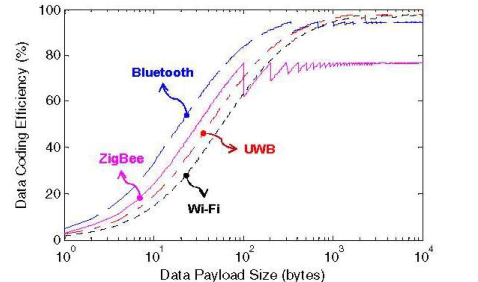
\includegraphics[width=1\textwidth]{datacodingefficieny}
   \caption{Comparision of the data coding efficiency for each protocol, found in \cite{comparitivestudywirelessprotocols}.}
   \label{fig:protocolefficiency}
\end{figure}

Figure \ref{fig:protocolefficiency} illustrates the data coding efficiency for each protocol. Bluetooth for example has the best data coding efficiency when using a small amount of bytes (around 339 bytes). Wi-FI and UWB on the other hand are more efficient for large data sizes. Where Zigbee saturates on 80 percent efficiency when the data size increases.\\

\textbf{Interference}\\
The ISM frequency band is used for industrial, scientific and medical purposes. This means that some regions of the frequency band can be used for educational purposes. All of the discussed protocols use techniques to overcome interference. Some frequency bands are nowadays (over)crowded. This is because of the succes of some of the frequency band regions. \cite{Bluetoothwifisurveyandcomparison} The 2,4 and 5,0 GHz bands for example full fill the needs of a lot appliances.

Ultrawideband operates in the 3.1 - 10.6 GHZ range. This region is used by satellites, radars, broadband wireless and wireless networks. Wi-Fi, ZigBee and Bluetooth operate in the 2,4 GHZ band. Appliances who also use this band are: Microwave ovens, homeRF devices and cordless phones. The 5GHz band is also used by Wi-Fi, which is less crowded. Zigbee also has another band to transmit to, the 915 MHz band which is used by simple sensor networks.

As mentioned before all of the protocols use techniques to counter interference from itself or neighbouring devices. Bluetooth's frequency hopping is less sensitive for strong narrow band interference, which only affects a few channels. Wi-Fi however is less sensitive to wide-band noise. \cite{Bluetoothwifisurveyandcomparison} Comparing the protocols, Ultra wideband has the best characteristics. The protocol has a wide bandwidth and the transmit power is low. It also interferes the least with other common appliances.\\

\textbf{Power consumption}\\
The power consumption of each protocol depends on the used hardware. To make a valid comparison, the paper \cite{comparitivestudywirelessprotocols} made a selection of average hardware. The comparison in figure \ref{fig:protocolenergy} gives an indication of the average power consumption of each protocol. Bluetooth and ZigBee both consume about 100 mW where the power consumption of UWB and Wi-Fi is about 700 mW. Figure \ref{fig:protocolefficiency} gives the normalized energy consumption of each protocol. The normalized energy is given in mJ/Mb. The normalized energy consumption indicates that ZigBee and Bluetooth both use more energy to send and receive the same amount of information. UWB is the most efficient protocol to process information.

\begin{figure}[H]
   \centering
   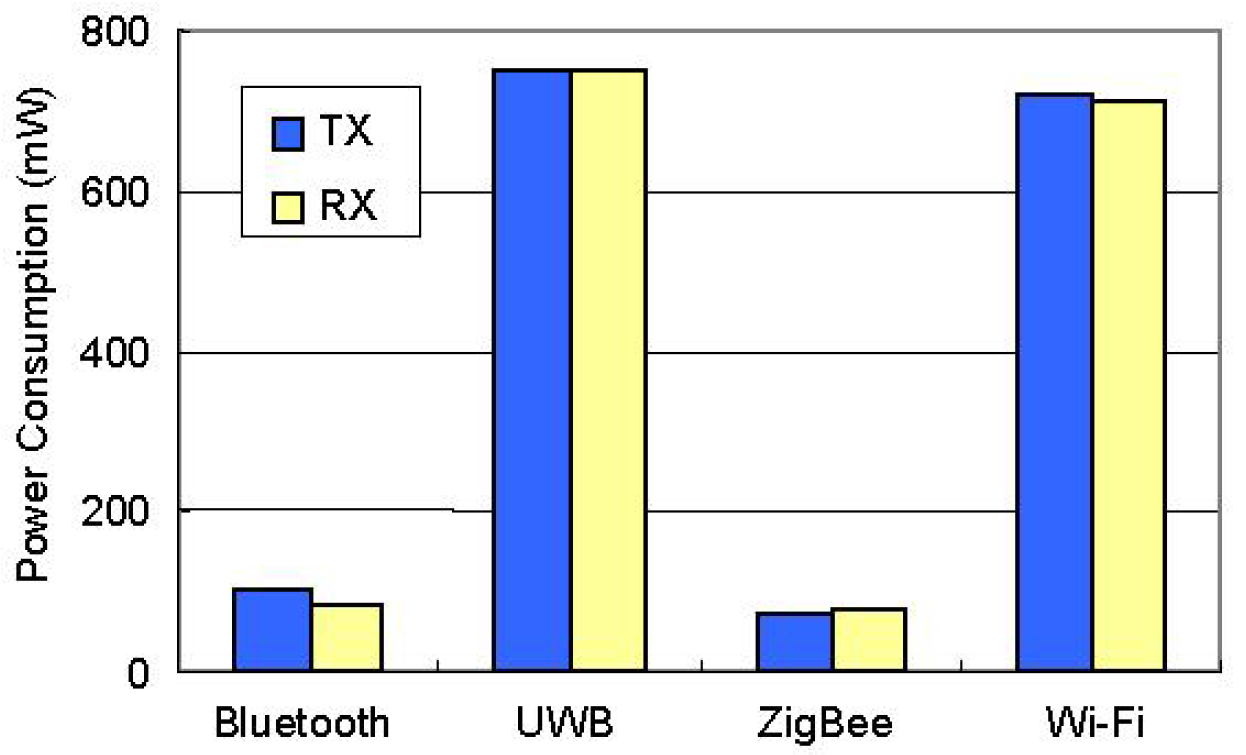
\includegraphics[width=1\textwidth]{images/protocolenergy.png}
   \caption{Comparision of the power consumption for each protocol, found in \cite{comparitivestudywirelessprotocols}.}
   \label{fig:protocolenergy}
\end{figure}

\begin{figure}[H]
   \centering
   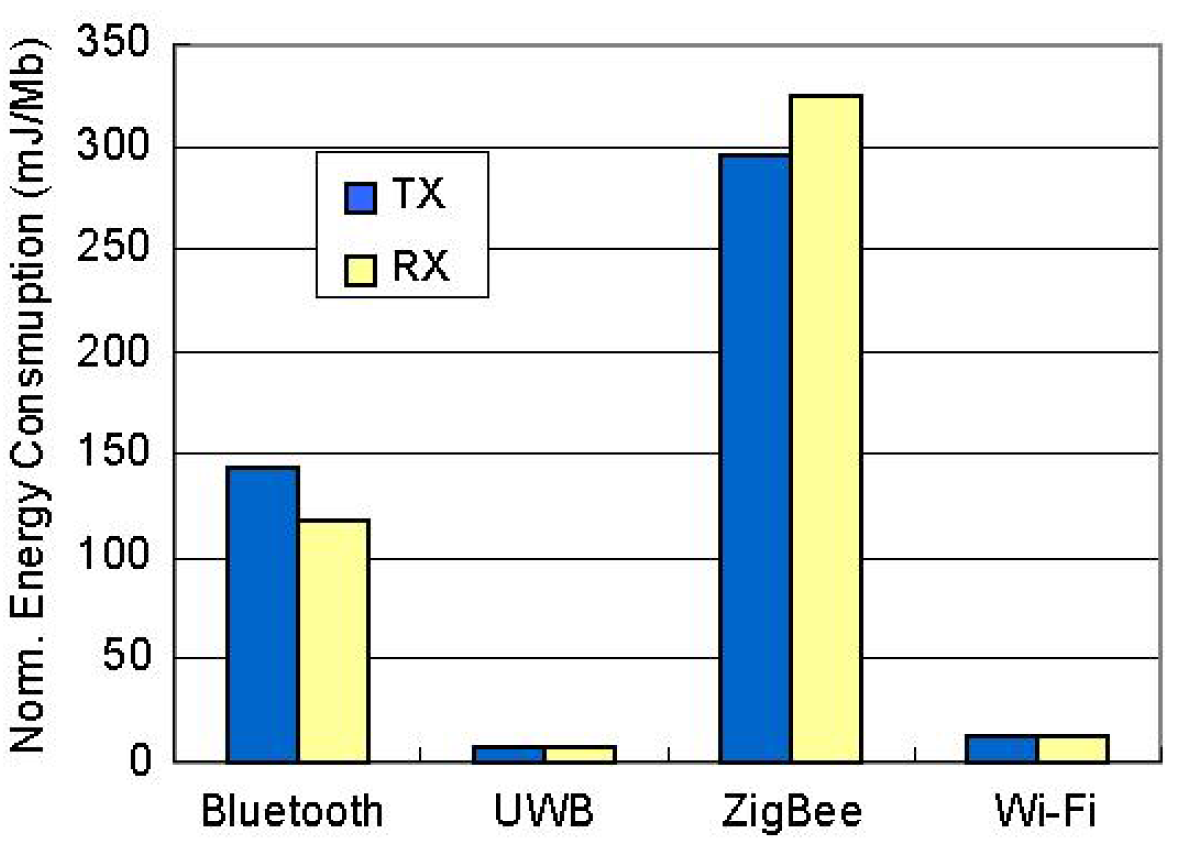
\includegraphics[width=1\textwidth]{images/protocolenergynormalized.png}
   \caption{Comparision of the normalized energy consumption for each protocol, found in \cite{comparitivestudywirelessprotocols}.}
   \label{fig:protocolenergynormalized}
\end{figure}


\paragraph{Conclusion comparison}
The final comparison is made in table \ref{protocolcompare}. There have been some adjustments in naming the characteristics to make the table fit the page. 'Rate' is the transceiving data rate, 'Range' is the transceiving data range, 'Scalability' of the protocol on large and small scale projects, 'Efficiency' means the data coding efficiency, 'Complexity' is the protocol complexity, 'Capacity' stands for the data distribution per square meter, 'Consumption' means the energy consumption.

\begin{table}[H]
\centering
\caption{The comparison of the protocols. The characteristics of each of the protocols get evaluated. The scoring is based on a number between zero and one, where zero is bad and one is good. The total score gives the best protocol for this situation.}
\label{protocolcompare}
\resizebox{\textwidth}{!}{\begin{tabular}{|l|c|c|c|c|c|c|c|c|c|}
\hline
\textbf{Protocol}  & \textbf{Rate} & \textbf{Range} & \textbf{Scalability} & \textbf{Efficiency} & \textbf{Complexity} & \textbf{Capacity} & \textbf{Interference} & \textbf{Consumption} & \textbf{Total} \\ \hline
\textbf{Wi-Fi}     & 1               & 1             & 0.75                   & 0.7                   & 0,75                  & 0.1                 & 0.5                     & 1                      & 5.8              \\ \hline
\textbf{Bluetooth} & 0               & 0                & 0                      & 1                     & 0                     & 0                   & 0.75                    & 0.25                   & 2                \\ \hline
\textbf{ZigBee}    & 0               & 1              & 1                      & 0.9                   & 1                     & 0.1                 & 0.5                     & 1                      & 5.5              \\ \hline
\textbf{UWB}       & 1               & 0                & 1                      & 0.8                   & 0.5                   & 1                   & 1                       & 0.25                   & 5.55             \\ \hline
\end{tabular}}
\end{table}

The information from table \ref{protocolcompare} results in the graph in figure \ref{fig:protocolcomparison}. The protocol with the highest score has the best characteristics to apply in the swarm network. The conclusion is that Wi-Fi is the best option followed by UWB, ZigBee and Bluetooth. The results of the comparison differ not much from each other. 

It is possible to create an wireless mesh network with all three of the protocols, however all of them have their own benefits and disadvantages. The preference depends on the available implementations which is discussed in a following chapter.

\begin{figure}[H]
   \centering
   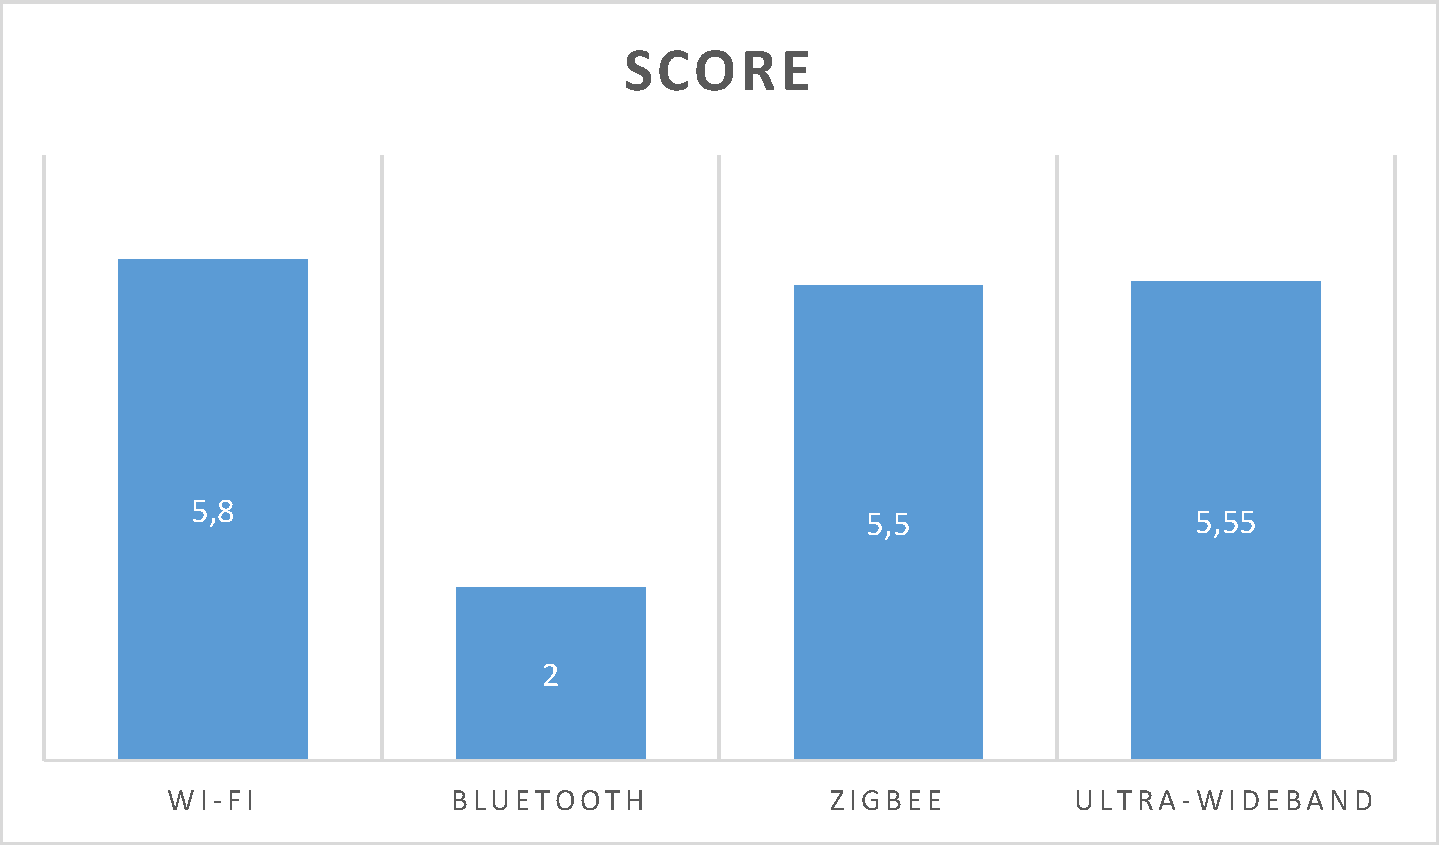
\includegraphics[width=1\textwidth]{protocolcomparison}
   \caption{Total scores for each reviewed protocol.}
   \label{fig:protocolcomparison}
\end{figure}


\newpage
\subsection{Conclusion communication}
In this section an sub-study in swarm communication is made. The results of the sub-study have resulted in recommendations for the implementation of the swarming module. An enumeration of the recommendations are given below:
\begin{itemize}
\setlength\itemsep{0em}
    \item The connection must be wireless due to the mobility of swarm members.
    \item A (partially connected) mesh network topology satisfies the desired network requirements.
    \item The network must be reliable, so it must use self-organization and topology control algorithms. \cite{WMN1}
    \item In a wireless network the single-path strategy for data distribution is preferred because of the power and bandwidth limitations. \cite{position-based}
    \item ART or MART can be used to address the nodes in a mesh network.
    \item Greedy routing or a derivative is the most suitable routing strategy.
    \item Scaling on large-scale projects is not possible without using geographic locating (precize locating). \cite{geographicalrouting}\cite{scalablelocation}. 
    \item The most suitable communication protocol in the described situation depends on the available implementation possibility. Wi-Fi, UWB and ZigBee are all three qualified to provide a wireless mesh network.
\end{itemize}

\newpage

\section{Proximity sensor}
For close range obstacle avoidance (0 m - 0,3 m, the robots will need some kind of proximity sensing technique. The sensor needs to differentiate between different "treats" for the robot to function properly. For example; when the sensor detects a small hill, which the robot can move over it should not trigger the robot to move away from it. But when it detects a big obstacle it should trigger the robot to move away. This is important because the robots will eventually be expected to move across rough terrain (like Mars). In the next paragraphs some different proximity sensor techniques will be discussed. Price is also a important factor while comparing these techniques. Multiple robots must be made on a tight budget, so costs should be cut where possible.\\

\subsection{Ultrasonic sensor}
Ultrasonic sensors are widely used in robotics for proximity sensing. An ultrasonic sensor uses the time of flight (TOF) to operate. It sends out an ultrasonic sound wave and measures the time it takes for the sound to be reflected back. The speed of the sound is known so the distance can be calculated. The fact that this method uses sound is a big advantage when measuring small distances. Sound has a velocity of propagation of around 340 m/s. Most other methods use signals that travel with the speed of light ( $3\cdot10^{8}$). The problem with the high velocity of  propagation especially with measuring distances shorter than one meter is that the TOF will be in terms of a few nanoseconds.  The hardware needed to process signals with this kind of speed will require more complex circuit design and ultimately cost more. The ultrasonic signal that is received after reflected from an object hold information about the shape and size of the object. This can be used to discriminate between different obstacles\cite{ultraobject}. Because there's a diffrent atmosphere on Mars ultrasonic sound gets heavily dappened \cite{soundonmars}. This mean that this method wont be usable on Mars itself. A pro of the ultrasonic sensor is the low cost. A sensor with specified for short distances costs between 2\euro and 10\euro.


\subsection{Lidar sensor}
Light detection and ranging (lidar) works with the same principle as the ultrasonic sensor. It uses time of flight to determine the distance from an object. Instead of sound it uses the light of a laser as its medium. Lidar can be used for various applications like: 3D modeling of an environment, weather forecast and distance measurements \cite{whatlidar}. Lidar is a proven technology on Mars, it has been used on the Phoenix mission to measure clouds and atmospheric dust \cite{lidarmars}. A lidar suitable for the purpose of proximity sensing would be de Lidar lite v2. This is a proximity sensor designed for robotics. It has a range 0-40 m and an accuracy of +/- 0,025 m. Being the cheapest lidar sensor on the market it still costs 100\euro. Object discrimination with the Lidar lite is not possible due to the limited information. More complex lidar systems with a moving laser could be able to discriminate and detect objects really precise, but this requires really complex systems.


\begin{figure}[!ht]

  \centering
      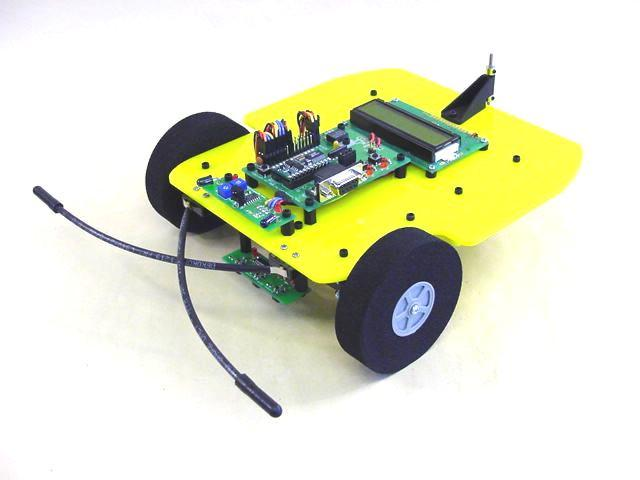
\includegraphics[width=0.5\textwidth]{voelsprieten.jpg}
  \caption{Robot met mechanische proximity sensor}  \label{voelspriet}
 
\end{figure}

\subsection{Mechanische sensor}
A mechanical sensor will consist of two important parts. The actuator, this could be a simple switch sensitive to a certain pressure. And the so called "arm" or "bumper", this is the part that makes contact with the obstacle's surface and works the mechanical force on the actuator. The beauty of this system is it's simplicity. There's no fast signals with different frequencies to be processed, just a simple on or of signal is all that needs to be observed. Due this limited input object discrimination wont be possible. Also robots bumping into object and each other is not a preferable situation. The robots might get stuck or break down.

\subsection{Sensor choice for the robot}
Now the question is which of the different sensor techniques proposed, is the best to implement on the swarm robots. While answering this question the following points will be taken into account:

\begin{itemize}
\setlength\itemsep{0em}
    \item The sensor must be easy to reproduce because multiple robots must be made from the swarm.
    \item The budget is limited, therefore the sensor price should be cheap compared the the total price of one robot.
    \item Energy usage should be as low as possible to increase the operation time per robot.
    \item For budget reasons there has been chosen to not take into account if the sensor would work on Mars.
    \item It must be possible to discriminate between different obstacles.
\end{itemize}

Looking at these points it becomes clear that the lidar sensor wouldn't be the best choice. It doesn't really have any outstanding pros compared to the other two techniques and it's much more expensive. . As talked about before the mechanical sensor has a few drawbacks compared to the ultrasonic sensor. For these reasons the ultrasonic sensor seems the best choice. The only issue left to solve is how to sense the difference between obstacles which the robot has to avoid, and things the robot doesn't have to avoid, but still might be detected by the sensor. This will be discussed in the next paragraph.

\subsection{Obstacle discrimination with an ultrasonic sensor}
An ultrasonic sensor is usually used to detect if there is some obstacle in the way. In this case there is made no difference made between a obstacle that the robot can move over, or a obstacle that should be avoided. For example: a small slope or hill might be detected as an obstacle, but in truth the robot can move over it. The robots developed for this program will eventually be able to cross harsh terrain. In this case the proximity sensor will need to discriminate between these situations. Working with ultrasonic waves there are multiple domains to work with. These are time, frequency and amplitude. Time is used to determine the distance between the object and the sensor. The change in frequency and/or amplitude contains information about the shape of the object\cite{ultraobject}see figure \ref{ultrafreq}. In the paper "Object recognition with ultrasonic sensor" is concluded that looking at the amplitude over time contains enough information to discriminate between object\cite{ultraobject}. The example is given of an object with separated surfaces of 3,5 cm, the echo from the second surface will be delayed by 0,2 milliseconds relative to the echo from the first surface. This delay can be easily detected with a microprocessor. The reason looking at frequency isn't the first choice is because of the higher hardware requirements it would require to properly sample the ultrasonic signal. Looking at amplitude and time does not require the signal to be sampled at the Nyquist rate so lower clock rate microprocessors can be used to do the processing.
\\
\begin{figure}[h]
  \centering
      \includegraphics[width=1\textwidth]{ultrafreq.pdf}
  \caption{The left graph shows the average PSD from 50 echos generated by a plastic botthle from a distance of 100cm, the average envelope is generated using 50 echos of the same bottle} \cite{ultraobject}  \label{ultrafreq}
\end{figure}
\newpage

\section{Swarmdetection}
\subsection{algorithm}
Using the radio communication and the microphones on the swarming units it is possible to determine the distance and angle of every unit within range. each robot will send out a broadcast saying it is going to send its detection signal. As soon as the other units receive this message they will start a timer. Immediately after the broadcast the broadcasting robot will send out a detection sound. As soon as this signal is received by the other robots' microphones the timer will stop and the different times of detection of each microphone will be used to calculate the angle and distance of the unit.
Using triliteration it is possible to determine the angles of the created triangle knowing the lengths. It is possible to calculate six angles, because of this it is possible to detect the direction of the broadcaster without the possibility of mirroring. As soon as the direction is know it becomes possible to put the detected robot on an XY grid using the build in compass. When all the robots within swarming range have done this all the relative positions will be know from each other.
\newpage

\section{Functional design}

This chapter describes the functional design of the swarming module. An overview of the swarming module is given in figure \ref{overall}. The module is designed in such a way that it is modulair. This module can be placed on an object (i.e. a robot) and can be used by the object to send and receive relevant information about other in-range swarming modules.

This chapter discusses the following subjects:
\begin{itemize}
\setlength\itemsep{0em}
\item Swarming module
\item Power supply and safety
\item Central operating unit
\item Wireless communication module
\item Relative orientation sensor
\item Orientation sensor
\item Localisation sensor
\end{itemize}

\subsection{Swarming module}
The overall design of the swarming module is shown in figure \ref{overall}. Each block of the overall design is described in the following figures.
\begin{figure}[h]
  \centering
      \includegraphics[width=1\textwidth]{overall.pdf}
  \caption{Overview of the swarm module design}
  \label{overall}
\end{figure}

\subsubsection{Power supply and safety}
An external power supply is used to provide the system of power. The system uses a fuse as a safeguard to protect the module's sub systems from overloading. The safeguard and power supply are shown in table \ref{power-supply} and \ref{safeguard}.

\begin{table}[H]
\centering
\caption{Power supply}
\label{power-supply}
\begin{tabular}{|p{1,5cm}|p{9,5cm}|}
\hline
Module   & Power supply                                        \\ \hline
Input    & 5 VDC, 3A                                            \\ \hline
Outputs  & 5 VDC, 3A                                             \\ \hline
Function & Provides the system with enough current to power all of the sub modules. \\ \hline
\end{tabular}
\end{table}

\begin{table}[H]
\centering
\caption{Safeguard}
\label{safeguard}
\begin{tabular}{|p{1,5cm}|p{9,5cm}|}
\hline
Module   & Safeguard                                        \\ \hline
Input    & 5 VDC, 3A                                            \\ \hline
Outputs  & 5 VDC, 3A                                             \\ \hline
Function & Protects the module with a fuse from overloading. \\ \hline
\end{tabular}
\end{table}

\subsubsection{Central operating unit}
The central operating unit processes data from the sensors and swarm network. This unit uses the external wireless swarm communication, the local communication bus and the debug interface as an communication channel. The local communication bus uses a TWI (Two Wire Interface) protocol and is used for the communication with the robots peripherals i.e. actuators. The debug interface of the central operating unit uses an UART protocol to communicate with external systems for debug purposes.

\begin{table}[H]
\centering
\caption{Central operating unit}
\label{cou}
\begin{tabular}{|p{1,5cm}|p{9,5cm}|}
\hline
Module   & Central operating unit                                        \\ \hline
Input    & 3,3 VDC \\
         & Data streams (TWI, UART)                                           \\ \hline
Outputs  & Data streams (TWI, UART)                                             \\ \hline
Function & Calculates the relative position to other swarming modules. Distributes local and external data streams. Analyses and uses sensor information.\\ \hline
\end{tabular}
\end{table}

\subsubsection{Wireless communication module}
The wireless communication module is reponsible for the wireless communication to other swarming modules. The specification of this block is given in table \ref{wcm}.

\begin{table}[H]
\centering
\caption{Wireless communication module}
\label{wcm}
\begin{tabular}{|p{1,5cm}|p{9,5cm}|}
\hline
Module   & Wireless communication module                                       \\ \hline
Input    & 5 VDC\\ 
        & Swarm data\\
        & RF signal                                              \\ \hline
Outputs  & RF signal                                           \\ 
& Swarm data \\ \hline
Function & Processes information to and from other swarm modules. Transmission speed is not defined yet. The transmission range must be around 100 meters or more. \\ \hline
\end{tabular}
\end{table}

\subsubsection{Orientation sensor}
The module uses an orientation sensor to calculate the relative position to other modules. This sensor is connected to the central operating unit which uses the sensor information for the localization algorithm. The specifications of the orientation sensor is given in table \ref{orisensor}.

\begin{table}[H]
\centering
\caption{Orientation sensor}
\label{orisensor}
\begin{tabular}{|p{1,5cm}|p{9,5cm}|}
\hline
Module   & Relative orientation sensor                                        \\ \hline
Input    & 5 VDC                                             \\ \hline
Outputs  & Orientation information                                           \\ \hline
Function & Retrieves the relative orientation of the module. Resolution of at least 45 degrees. \\ \hline
\end{tabular}
\end{table}


\subsection{Short range localisation sensor}
The principle of the short range localisation sensor is displayed in figure \ref{demodulator}, \ref{modulator} and \ref{pll}.



As mentioned earlier the short relative distance measurement will be done acoustically. With acoustic sensing it is required to let the speaker sway to the right oscillation frequency, reaching this oscillation frequency takes time since the speaker won’t oscillate at the right frequency instantly. This complicates the measurement a little bit, since just detecting the to be measured signal won’t always translate into an exact distance due to the time the speakers take to sway into oscillation.

A solution to this problem is to create a fixed reference point within the sent signal. Creating this reference point after a fixed time enables the speaker to sway into oscillation making sure that no faulty measurements occur do to this “swaying time”. When the reference point has been detected by the receiver an accurate distance can be determined by subtracting the fixed “sway time”.

Without the implementation of this fixed reference point it is possible for a receiver to miss a few periods of the signal, due to the speaker still swaying into oscillation and the time of swaying being unknown. For example take an acoustic signal (Speed of sound 340.29 m/s) with a frequency of 4000Hz, one period of this signal is 0.00025s. Missing one period of this signal translates into a distance error of 8.5cm. Since the sway time of a speaker can change over time due to mechanical stresses a fixed time stamp seems the most suitable solution for the long term.

\subsubsection{Modulation}

The audio signal will be modulated with frequency shift keying which is an FM based modulation technique. This modulator exist of an voltage controlled oscillator (VCO) with a center frequency of 4KHz. The VCO sends out 3,9KHz when no voltage is applied to it and 4,1KHz when 5V is applied to it. This gives the VCO a frequency swing of 200Hz at which 3,9KHz means a logic ‘0’ and 4,1KHz means a logic ‘1’. This frequency will be fed to an audio amplifier connected to the speaker. See figure \ref{modulator} for a schematic representation of the modulator.

\begin{figure}[H]
  \centering
      \includegraphics[width=1\textwidth]{modulator.pdf}
  \caption{Modulator}
  \label{modulator}
\end{figure}

\subsubsection{Demodulation}

A demodulator will be needed to retrieve the digital signal send from one swarm-module to another.  One swarming module will send an acoustic signal to the other modules, this signal will then be picked up by an sensor and will need to be processed properly before it can be used to determine the time it took the acoustic signal to travel from one swarming-module to the other. The signal retrieved by the acoustic sensor will also pick up a lot of noise and other sounds from the environment. Also, when further away the signal might be low in amplitude. To increase the amplitude and lower the noise, the signal will be amplified and bandwidth filtered. These modifications to the signal will improve the signal to noise ratio drastically but a lot of noise might still remain. Therefore the demodulator itself must be insensitive to noise.  
The main purpose is the demodulator is to identify the reference point. And more importantly, determine the point in time the reference point is spotted. The time determined will be used to calculate the distance. Hence, the precision in which the demodulator determines the reference point in time effects the precision of the distance measurement. Only one swarming module will be sending his acoustic signal at any moment. When there are 10 units in its specified range and a preferred update frequency of 40Hz (see section 1). This gives every swarming-module only a small window in time to send their signal and for the other to receive it. When a frequency of 4kHz is chosen for the signal, every swarming-module will have 10 periods to send their signal. There for the demodulator must be able to lock onto the signal and determine the reference point within a few periods of the acoustic signal. See figure \ref{demodulator} for a schematic representation of the demodulator.

\begin{figure}[H]
  \centering
      \includegraphics[width=1\textwidth]{demodulator.pdf}
  \caption{Demodulator}
  \label{demodulator}
\end{figure}

\begin{table}[H]
\centering
\caption{Demodulation specifications}
\label{demosensor}
\begin{tabular}{|p{1,5cm}|p{9,5cm}|}
\hline
Module   & Demodulator                                   \\ \hline
Input    & Modulated signal                                             \\ \hline
Outputs  & Demodulated signal                                         \\ \hline
Function & Demodulation \\ \hline
Features & Noise insensitive, precision (time), Quick demodulation  \\ \hline
\end{tabular}
\end{table}


\subsection{long range distance measurement}
The long range distance measurement is defined as 3m to 25m(section 1.2). The main reason for the long range distance measurement is for units out of the close range area to be able to find the swarm again. In section 1.2 its restricted to a maximum distance of 25m, but implementations that can achieve a longer range are preferred. As stated before the long range angle measurement will fall out of the scope of this project. Robots will need to use a smart algorithm to find the right way to the swarm. In section 1.2 the following specification are determined: maximum deadzone of two meters, minimal update frequency of 1Hz and a maximum deviation of +/- 1 meter.

\begin{table}[H]
\centering
\caption{long range distance sensor specifications}
\label{longrangesensor}
\begin{tabular}{|p{1,5cm}|p{9,5cm}|}
\hline
Module   & Long range distance sensor specifications                          \\ \hline
Input    & 5V DC                                           \\ \hline
Outputs  & Relative distance from other modules                                        \\ \hline
Features & Rough estimate of relative distance, relative big deadzone, low update frequency  \\ \hline
\end{tabular}
\end{table}


\newpage

\section{Technical design}
 
In this section the technical design of the swarm module will be discussed. The same structure that was used in the function design will be used here. The design choices that are made will be explained. The following sections will be looked at: 


\begin{itemize}
\setlength\itemsep{0em}
\item Swarming module
\item Power supply and safety
\item Central operating unit
\item Wireless communication module
\item Relative orientation sensor
\item Orientation sensor
\item Localisation sensor
\end{itemize}

\subsection{Swarming module}

The overall design of the technical implementation of the swarming module is shown in figure (nog in te vullen). 

Hier mooi blokschemaatje toevoegen. 


\subsubsection{Power Supply and Safety}

\subsubsection{Central Operation Unit}

\subsubsection{Wireless Communication module}

For the wireless communication module the most important function is that it can transmit information over atleast 100 meters. The speed of de communication is not defined yet. The Swarmbee LE module will be used for the wireless communication. Its uses the ISM band, 2.4 GHz to transmit the data. The maximum range of the module relies on the environment in which it is used. Under ideal conditions the Swarmbee can reach a distance of 1200 meters. It depends on how many obstacles, reflections and interference there is to disturb the signal. An experiment from Nanotron showed that until a range of 150 meters the ranging success rate is about 100\%. The host interfaces uses UART with a transmission speed of 155 kbps. Transmitting data between the swarm modules can be configured with a speed of 250 Kbps or 1 Mbps. This module fits all the specifications and is suitable for the use of wireless communication. 


\subsubsection{Orientation sensor}

\subsection{Localisation sensors}


\subsubsection{Short Range}




\subsubsection{Long Range}

For the long range localization, the distance needs to be determined between atleast 3 to 25 meters, with an accuracy of 1 meter. It should be updated with a frequency of 1 Hz. In the Swarmbee module there is already a localization function implemented. This localization function is not usable for short distances but should suit the requirements for the long distance localization. The localization has an accuracy of atleast 30 centimetres and can update with a frequency of 1 Hz. The only downside of this function that is cant determine what angle the signal comes from, it only estimates the distance from the source to the receiver. The modules uses Time of Arrival to determine the distance. All these specifications meet the requirements that are needed, thus this module suits the functionality. 




\section{Bibliografie}
\bibliography{references}
\bibliographystyle{IEEEtran}



\end{document}
